\documentclass[12pt, letterpaper]{article}
\usepackage[utf8]{inputenc}
\usepackage[T1]{fontenc}
\usepackage{newtxtext,newtxmath}
\usepackage[spanish]{babel}
\usepackage{algorithmic}
\usepackage{graphicx}
\usepackage{textcomp}
\usepackage{xcolor}
\usepackage{url}
\usepackage{float}
\usepackage{geometry}
\geometry{letterpaper, margin=2.54cm}
\usepackage{setspace}
\singlespacing
\usepackage{indentfirst}
\setlength{\parindent}{1.27cm}
\usepackage{titlesec}
\usepackage[round]{natbib}

\titleformat{\section}{\normalfont\normalsize\bfseries\centering}{}{0em}{}
\titleformat{\subsection}{\normalfont\normalsize\bfseries}{}{0em}{}

\usepackage{fancyhdr}
\pagestyle{fancy}
\fancyhf{}

\fancyhead[L]{\MakeUppercase{Limitaciones del turismo digital actual}}
\fancyhead[R]{\thepage}

\renewcommand{\headrulewidth}{0pt}

\fancypagestyle{plain}{
  \fancyhf{}
  \fancyhead[L]{\MakeUppercase{Limitaciones del turismo digital actual}}
  \fancyhead[R]{\thepage}
  \renewcommand{\headrulewidth}{0pt}
}
\begin{document}

\begin{center}
\textbf{Transformación Digital del Sector Turístico: Plataforma Inteligente para la Planificación Integrada y Colaborativa de Viajes}
\end{center}

\begin{flushright}
\vspace{1em}
Santiago Amaya Zapata\\
Ricardo Ayala Garzon\\
Santiago Botero García
\end{flushright}

\vspace{1em}
\noindent\textbf{Resumen}

El presente artículo describe una solución empresarial de transformación digital para el sector turístico, concebida como ecosistema de software modular y distribuido: cliente web (\textit{React}), cliente móvil nativo (\textit{Android, Kotlin}), núcleo transaccional (\textit{Java Spring Boot}), microservicio de inteligencia artificial (\textit{Python FastAPI}) y capa de despliegue en \textit{Amazon Web Services (AWS)} definida en el repositorio de infraestructura del proyecto (API Gateway, Application Load Balancer, grupos de autoescalado sobre EC2, RDS PostgreSQL, S3, SNS, SQS, CloudFront y CloudWatch). La solución se fundamenta en una arquitectura cognitiva que combina IA no exclusivamente conversacional, sistemas de recomendación híbridos y modelos de optimización para personalización y gestión de recursos. Como diferenciador de valor, incorpora \textit{viaje social colaborativo} alineado con la documentación de requisitos ágiles del repositorio: perfiles de viajero, intención de viaje, coincidencias por destino y fechas, conexiones, mensajería y agenda compartida, evolucionando hacia \textit{matching} multidimensional. Se presentan modelo de negocio digital, arquitectura de referencia reproducible por scripts, marco metodológico \textit{data-centric} y métricas de impacto, mostrando cómo la transformación digital genera valor para el ecosistema turístico colombiano.

\textit{Palabras claves:} Transformación Digital, Arquitectura Empresarial, Sistemas Distribuidos, Inteligencia Artificial, Optimización de Operaciones, Turismo Digital, Colaboración Social, PEAS, Modelo de Negocio Digital.

\vspace{2em}
\begin{center}
\textbf{Digital Transformation in Tourism: Enterprise Platform for Integrated and Collaborative Travel Planning}
\end{center}

\noindent\textbf{Abstract}

The digital transformation of the tourism sector represents a strategic opportunity for enterprise solutions that optimize operational efficiency and customer experience. Colombia projects over 21.7 million visitors by 2025, with sector growth exceeding 6\% \citep{ref1}, yet fragmentation across transportation, accommodation and activities creates inefficiencies. Many offerings rely on conversational generative models without deep integration into core transactional and analytical paths. This paper presents a generic enterprise digital transformation architecture whose reference deployment is specified in the project's infrastructure repository: a React web client served via S3 and CloudFront, an Android (Kotlin) mobile client, a Spring Boot core API, a FastAPI AI microservice, Amazon API Gateway and an Application Load Balancer routing to EC2 Auto Scaling groups, PostgreSQL on Amazon RDS, object storage on S3, asynchronous integration via SNS and SQS, and observability with CloudWatch---together with hybrid recommenders, supervised learning and cognitive-memory framing. The differentiator is a \textit{social travel ecosystem}: traveler matching, collaborative itineraries and community engagement. Expected impact includes better operational decisions through analytics, personalization, seasonality-aware recommendations and network effects. The contribution links research-oriented AI narratives to a concrete, modular AWS deployment model suitable for academic lab constraints.

\textit{Keywords:} Digital Transformation, Enterprise Architecture, Distributed Systems, Artificial Intelligence, Operations Optimization, Digital Tourism, Social Collaboration, PEAS, Digital Business Model.

%================================================================================
\section*{Introducción}
%================================================================================

\subsection*{Contexto general}

La transformación digital del sector turístico ha generado oportunidades para plataformas integradas que optimicen la experiencia del viajero. Colombia proyecta cerrar el 2025 con más de 21,7 millones de viajeros, consolidando un crecimiento superior al 6 \% en el sector \citep{ref1}, impulsado por la conectividad aérea y la confianza de los usuarios \citep{ref2}. El turismo digital se apoya en tecnologías emergentes como la computación en la nube, el análisis de grandes volúmenes de datos y la inteligencia artificial.

\subsection*{Planteamiento del problema empresarial}

La fragmentación operativa del sector turístico genera ineficiencias significativas: los operadores de transporte, alojamiento y actividades operan en silos aislados, impidiendo la optimización conjunta de capacidad y experiencia. Desde la perspectiva empresarial, esta desconexión resulta en subutilización de capacidad, estacionalidad extrema y pérdida de oportunidades de \textit{cross-selling}. Los sistemas actuales dependen predominantemente de modelos generativos conversacionales que no se integran con los procesos transaccionales y analíticos centrales, limitando mejoras operativas medibles. El problema fundamental es la ausencia de una solución empresarial modular que combine un núcleo de negocio (API REST), un microservicio de IA desacoplado, mensajería asíncrona entre componentes y clientes multiplataforma, mientras habilita colaboración explícita entre viajeros. Las plataformas comerciales existentes \textbf{no aprovechan de forma sistemática el valor de red generado por la colaboración entre usuarios}: la planificación suele ser individual, con pérdida de efectos de red y comunidad. Este enfoque limita la eficiencia operativa de los proveedores y el valor percibido por los viajeros.

\subsection*{Análisis del estado del arte empresarial}

Las soluciones tecnológicas actuales en el sector turístico presentan limitaciones significativas desde la perspectiva de la transformación digital empresarial:

\begin{itemize}
\item \textbf{Foco en interfaz versus integración operativa:} Las plataformas existentes priorizan la experiencia de usuario superficial sin integrarse con los sistemas de gestión operativa de los proveedores turísticos.
\item \textbf{Limitaciones en optimización matemática:} Carecen de formalización rigurosa que permita la optimización de recursos y la predicción precisa de demanda.
\item \textbf{Gestión ineficiente de la estacionalidad:} No implementan modelos predictivos avanzados para mitigar los efectos estacionales y optimizar la ocupación.
\item \textbf{Ausencia de estrategia de valor de red:} Ignoran el potencial estratégico de la colaboración entre usuarios como motor de lealtad y diferenciación competitiva.
\end{itemize}

Las soluciones comerciales predominantes ofrecen personalización básica pero carecen de la profundidad analítica y la integración operativa necesarias para generar transformación digital real. La ausencia de arquitecturas empresariales integrales limita su capacidad para optimizar la cadena de valor del turismo y crear ventajas competitivas sostenibles.

\subsection*{Oportunidad de transformación digital}

El contexto actual presenta una oportunidad estratégica para implementar una solución empresarial integral que transforme la cadena de valor del turismo. Se requiere una plataforma digital que: (i) exponga capacidades de negocio mediante APIs HTTP y contratos estables; (ii) incorpore un servicio de IA especializado (recomendación, compatibilidad entre viajeros) separado del núcleo transaccional; (iii) implemente modelos predictivos para gestión de estacionalidad y asignación de recursos; (iv) habilite colaboración entre usuarios (coincidencias, conexiones, coordinación de itinerarios) documentada en los requisitos ágiles del repositorio; (v) se despliegue sobre una arquitectura cloud-native reproducible (scripts de infraestructura, API Gateway, balanceador, cómputo elástico, RDS, S3, SNS/SQS, CloudFront, CloudWatch). Esta solución representa una transformación digital al alinear modelo de negocio, datos y despliegue modular.

%================================================================================
\section{Descripción y Caracterización del Problema}
%================================================================================

\subsection{Contexto específico}

El mercado turístico digital presenta alta competencia y una creciente demanda de experiencias personalizadas. Según informes oficiales del Ministerio de Comercio, Industria y Turismo (MINCIT) \citep{ref3}, así como estadísticas sobre visitantes no residentes \citep{ref4} y datos del DANE sobre el aporte del turismo al PIB nacional \citep{ref5}, se evidencia una tendencia sostenida de crecimiento en el sector.

\subsection{Impactos}

\begin{itemize}
\item \textbf{Sociales:} Los viajeros deben dedicar tiempo excesivo a planificar viajes dispersando la búsqueda entre múltiples sitios; la falta de personalización reduce la satisfacción con la experiencia turística. Además, la ausencia de mecanismos de conexión entre usuarios genera aislamiento en la planificación y limita las oportunidades de viajes colaborativos, a pesar de la demanda creciente de experiencias compartidas.
\item \textbf{Económicos:} La estacionalidad extrema genera picos de demanda en ciertas regiones y periodos, mientras otras zonas permanecen subutilizadas, afectando el retorno de inversión de los operadores turísticos.
\item \textbf{Técnicos:} La fragmentación de datos impide la construcción de perfiles unificados y recomendaciones coherentes; la ausencia de integración limita la optimización operativa.
\end{itemize}

\subsection{Métricas del sistema actual}

\begin{itemize}
\item \textbf{¿Cuántos turistas recibe Colombia?} Más de 3 millones en el primer semestre de 2025 \citep{ref6}; Bogotá superó 1,2 millones de visitantes internacionales entre enero y agosto de 2025 \citep{ref7}. \textit{Interpretación:} El volumen de demanda exige soluciones escalables.
\item \textbf{¿Cuáles son los desafíos estructurales?} Los desafíos del turismo en Colombia han sido analizados en estudios especializados \citep{ref8}; se proyecta que el país continúe consolidándose como destino global \citep{ref9}. \textit{Interpretación:} La competencia exige innovación tecnológica y diferenciación.
\end{itemize}

%================================================================================
\section{Objetivos}
%================================================================================

\subsection{Objetivo general}

Diseñar e implementar conceptualmente una solución empresarial de transformación digital para el turismo colombiano que articule planificación de viajes, datos transaccionales y un componente de viaje social colaborativo, apoyada en sistemas de recomendación híbridos, modelos predictivos para mitigación de estacionalidad y una arquitectura de despliegue en AWS acorde al repositorio de infraestructura del proyecto.

\subsection{Objetivos específicos}

\begin{itemize}
\item \textbf{Analizar} el estado del arte en sistemas de recomendación y arquitecturas cognitivas aplicadas al turismo digital.
\item \textbf{Diseñar} un dataset estructurado orientado al contexto turístico colombiano bajo enfoque data-centric.
\item \textbf{Formalizar} el modelo matemático del sistema híbrido de recomendación y de predicción de demanda.
\item \textbf{Implementar conceptualmente} la arquitectura de referencia sobre AWS según el repositorio de infraestructura: API Gateway, Application Load Balancer, EC2 con Spring Boot y FastAPI, RDS PostgreSQL, S3, SNS, SQS, CloudFront y CloudWatch.
\item \textbf{Evaluar} el desempeño del sistema mediante métricas predictivas (RMSE, MAE, Precision@K, Recall@K) y de impacto territorial.
\item \textbf{Diseñar} el módulo de conexión social (grupos de viaje, \textit{matching}, convocatorias abiertas) como componente diferenciador integrado en la arquitectura.
\end{itemize}

%================================================================================
\section{Marco Teórico}
%================================================================================

\subsection{Arquitectura Empresarial}

La arquitectura empresarial se entiende como la estructuración organizada de procesos, datos, aplicaciones e infraestructura tecnológica dentro de una organización \citep{ref12}. Los modelos contemporáneos incorporan enfoques de microservicios y arquitecturas \textit{event-driven}, lo que permite una mayor escalabilidad, flexibilidad y capacidad de integración entre sistemas, adaptándose a entornos dinámicos y cambiantes.

\subsection{Sistemas de Recomendación}

Los sistemas de recomendación se clasifican generalmente en tres categorías principales:

\begin{itemize}
\item \textbf{Basados en contenido:} sugieren ítems similares a aquellos previamente valorados por el usuario, utilizando características y descriptores de los ítems.
\item \textbf{Filtrado colaborativo:} se basan en el análisis de preferencias de múltiples usuarios para generar recomendaciones, detectando patrones de comportamiento similares.
\item \textbf{Modelos híbridos:} combinan enfoques de contenido y colaborativo para mejorar la precisión y reducir problemas como la escasez de datos o el sesgo de popularidad \citep{ref11}.
\end{itemize}

Formalmente, dado un conjunto de usuarios $U$ y un conjunto de ítems $I$, el objetivo es estimar la preferencia de un usuario $u$ sobre un ítem $i$ mediante:

\begin{equation}
\hat{r}_{ui} = f(u, i)
\end{equation}

donde $\hat{r}_{ui}$ representa la predicción de interés o valoración del usuario $u$ sobre el ítem $i$, y $f$ es la función de recomendación que puede incorporar técnicas de aprendizaje supervisado, heurísticas o modelos probabilísticos.

\subsection{Mitigación de Estacionalidad}

En turismo y servicios, la estacionalidad es un factor crítico que afecta la demanda. Esta puede modelarse mediante series temporales, como el modelo SARIMA \citep{ref10}:

\begin{equation}
\Phi_p(B)\Phi_P(B^s)(1-B)^d(1-B^s)^D y_t = \Theta_q(B)\Theta_Q(B^s)\epsilon_t
\end{equation}

donde $s$ representa el período estacional, $B$ es el operador de rezago, y los parámetros $(p,d,q,P,D,Q)$ ajustan la tendencia, estacionalidad y ruido de la serie temporal, permitiendo anticipar picos y valles de demanda.

\subsection{Modelo PEAS}

Desde la perspectiva de agentes inteligentes, un sistema racional toma decisiones que maximizan su desempeño según la información disponible y las condiciones del entorno. El modelo PEAS (\textit{Performance measure, Environment, Actuators, Sensors}) proporciona un marco formal para describir arquitecturas de agentes inteligentes.

\textbf{Performance Measure:} El desempeño del agente se evalúa mediante: precisión y relevancia de recomendaciones (Precision@K, Recall@K); tasa de conversión posterior a recomendaciones personalizadas; reducción del tiempo promedio de planificación de viaje; incremento en retención y recurrencia de usuarios; nivel de satisfacción (NPS y feedback explícito).

\textbf{Environment:} Entorno digital dinámico, parcialmente observable y no determinístico: usuarios con preferencias heterogéneas y capacidad de interacción entre sí; proveedores turísticos; variaciones en precios, disponibilidad y demanda estacional; factores externos (tendencias, eventos regionales). La \textbf{interacción usuario-usuario} (solicitudes de unión, formación de grupos, convocatorias abiertas) constituye una dimensión explícita del entorno que el sistema debe percibir y sobre la cual debe actuar.

\textbf{Sensors:} Datos de navegación (clics, búsquedas, tiempo de permanencia); historial de reservas y cancelaciones; preferencias declaradas; datos de ubicación y contexto temporal; tendencias externas y señales de mercado; \textbf{preferencias sociales y disposición para viaje colaborativo}; historial de interacción entre usuarios (grupos formados, solicitudes aceptadas o rechazadas, afinidades detectadas).

\textbf{Actuators:} Generación automática de itinerarios personalizados; recomendaciones priorizadas; alertas sobre cambios de precio o disponibilidad; \textbf{sugerencias de conexión entre usuarios con intereses similares}; \textbf{creación y gestión de grupos de viaje}; \textbf{invitaciones a viajes abiertos y solicitudes de unión}; ajustes dinámicos en visibilidad de destinos para mitigar estacionalidad.

%================================================================================
\section{Modelo de Negocio}
%================================================================================

El modelo de negocio se basa en una plataforma multisided que conecta usuarios y proveedores turísticos, y se fundamenta en estrategias de monetización diversificadas.

\subsection{Propuesta de Valor Empresarial}

La solución genera valor estratégico para múltiples stakeholders del ecosistema turístico:

\begin{itemize}
\item \textbf{Integración vertical de la cadena de valor:} Centralización de reservas, pagos y gestión de servicios en un ecosistema digital unificado, eliminando silos operativos.
\item \textbf{Optimización de recursos mediante IA:} Algoritmos predictivos para gestión de estacionalidad, asignación eficiente de capacidad y maximización de ingresos para operadores.
\item \textbf{Experiencia cliente hiper-personalizada:} Sistemas de recomendación híbridos que adaptan ofertas en tiempo real basándose en comportamiento histórico y contexto.
\item \textbf{Ecosistema de valor de red:} Plataforma colaborativa que habilita matching inteligente entre viajeros, formación de comunidades y efectos de red que generan lealtad y retención.
\item \textbf{Inteligencia de negocio avanzada:} Analítica predictiva para operadores turísticos, incluyendo pronósticos de demanda, optimización de precios y segmentación de mercado.
\item \textbf{Transformación de procesos operativos:} Automatización de flujos de trabajo, reducción de costos operativos y mejora en eficiencia de gestión.
\end{itemize}

\subsection{Modelo de Monetización Digital}

El modelo de negocio diversificado maximiza el valor capturado a través de múltiples streams de ingresos:

\begin{itemize}
\item \textbf{Comisiones transaccionales:} Porcentaje sobre reservas de transporte, alojamiento y actividades procesadas a través de la plataforma.
\item \textbf{Suscripciones empresariales:} Planes premium para operadores turísticos con analítica avanzada, herramientas de optimización y acceso prioritario a demanda.
\item \textbf{Servicios de inteligencia de negocio:} Dashboards analíticos, reportes de tendencias de mercado y consultoría basada en datos para toma de decisiones estratégicas.
\item \textbf{Marketplace de servicios complementarios:} Plataforma para proveedores de seguros, transporte local y experiencias personalizadas.
\item \textbf{Licenciamiento de tecnología:} API y componentes de IA para integración con sistemas existentes de grandes operadores turísticos.
\end{itemize}

\subsection{Cuantificación del Impacto}

El impacto financiero se mide mediante el Retorno sobre la Inversión (ROI):

\begin{equation}
ROI = \frac{Beneficio\ incremental - Inversion}{Inversion}
\end{equation}

%================================================================================
\section{Propuesta de Solución}
%================================================================================

\subsection{Solución Empresarial Integrada}

Se propone una solución empresarial de transformación digital que reestructura la cadena de valor del turismo mediante capacidades modulares. La solución implementa una arquitectura cloud-native con APIs HTTP, núcleo en Spring Boot, microservicio de IA en FastAPI y mensajería SNS/SQS, mientras habilita colaboración entre usuarios para efectos de red. El diferenciador es el \textbf{ecosistema de viaje colaborativo inteligente}: coincidencia por destino y fechas, solicitudes de conexión, mensajería, itinerarios y actividades compartidas, y evolución hacia \textit{matching} multidimensional, en línea con la documentación técnica del repositorio. Se incorpora IA en procesos de recomendación y compatibilidad, modelos matemáticos para optimización y predictivos para estacionalidad, y una infraestructura escalable documentada (EC2 con autoescalado, RDS, S3, orquestación perimetral con API Gateway y ALB). Los artefactos de contenedor y CI/CD en los módulos de código apoyan prácticas DevOps sin sustituir el modelo de despliegue descrito en la infraestructura de referencia.

\subsection{Arquitectura cognitiva (Memoria Episódica, Semántica y Procedimental)}

La arquitectura se estructura siguiendo una analogía con la memoria humana, dividiendo el sistema en tres tipos de memoria: episódica, semántica y procedimental.

\subsubsection{Memoria Episódica}

Almacena eventos históricos específicos del comportamiento de viajeros: historial de reservas, secuencias de navegación, interacciones sociales, cancelaciones y flujos estacionales. \textbf{Infraestructura implementada:} RDS PostgreSQL para eventos transaccionales; S3 para almacenamiento histórico de datos; SQS y SNS para captura y distribución de eventos en tiempo real. Modelos aplicados: algoritmos de series temporales y análisis de patrones implementados en el servicio IA con Python y Scikit-learn.

\subsubsection{Memoria Semántica}

Representa conocimiento estructurado del dominio turístico: taxonomía de destinos y actividades, segmentación de viajeros, relaciones entre regiones y patrones de comportamiento. \textbf{Infraestructura implementada:} RDS PostgreSQL para datos estructurados y relaciones; S3 para almacenamiento de modelos semánticos; procesamiento mediante el servicio IA. Modelos aplicados: algoritmos de clustering (K-Means), segmentación y análisis de cohortes implementados con Scikit-learn.

\subsubsection{Memoria Procedimental}

Define reglas de negocio y algoritmos de optimización: políticas de pricing dinámico, priorización de recomendaciones, optimización de itinerarios y estrategias de balanceo oferta-demanda. \textbf{Infraestructura implementada:} Microservicios desplegados en instancias EC2 con Auto Scaling; reglas de negocio implementadas en Spring Boot (backend) y FastAPI (servicio IA); caching local para decisiones en tiempo real. Modelos aplicados: sistemas híbridos de recomendación, algoritmos de optimización combinatoria y heurísticas de asignación de recursos.

\subsubsection{Plataforma de Colaboración Inteligente}

Este componente implementa un motor de valor de red alineado con las épicas y \textit{user stories} del repositorio de documentación: perfil mínimo de viajero, registro de intención de viaje, búsqueda de coincidencias por destino y fechas, solicitudes de conexión, mensajería entre conexiones, cronograma personal y actividades compartidas, y evolución hacia recomendaciones y \textit{matching} asistidos por IA. El sistema utiliza algoritmos de aprendizaje automático para compatibilidad multidimensional basada en preferencias declaradas, historial de comportamiento y disposición colaborativa. Las capacidades empresariales incluyen: \textbf{(i)} coordinación de grupos y planes compartidos; \textbf{(ii)} mecanismos de confianza y reputación a medida que madure el producto; \textbf{(iii)} extensiones de \textit{marketplace} colaborativo; \textbf{(iv)} analítica de patrones de conexión. El ecosistema genera efectos de red que aumentan el valor con cada usuario adicional.

%================================================================================
\section*{Arquitectura de la Solución y Tecnológica}
%================================================================================

La arquitectura de despliegue adopta como \textbf{fuente de verdad} la especificación del repositorio de infraestructura del proyecto: topología AWS con API Gateway, Application Load Balancer, instancias EC2 para el núcleo Spring Boot y el microservicio FastAPI, RDS PostgreSQL, S3, SNS, SQS, CloudFront y CloudWatch. Los clientes web (\textit{React}) y móvil (\textit{Kotlin}) consumen las APIs expuestas en ese perímetro.

\begin{figure}[H]
    \centering
    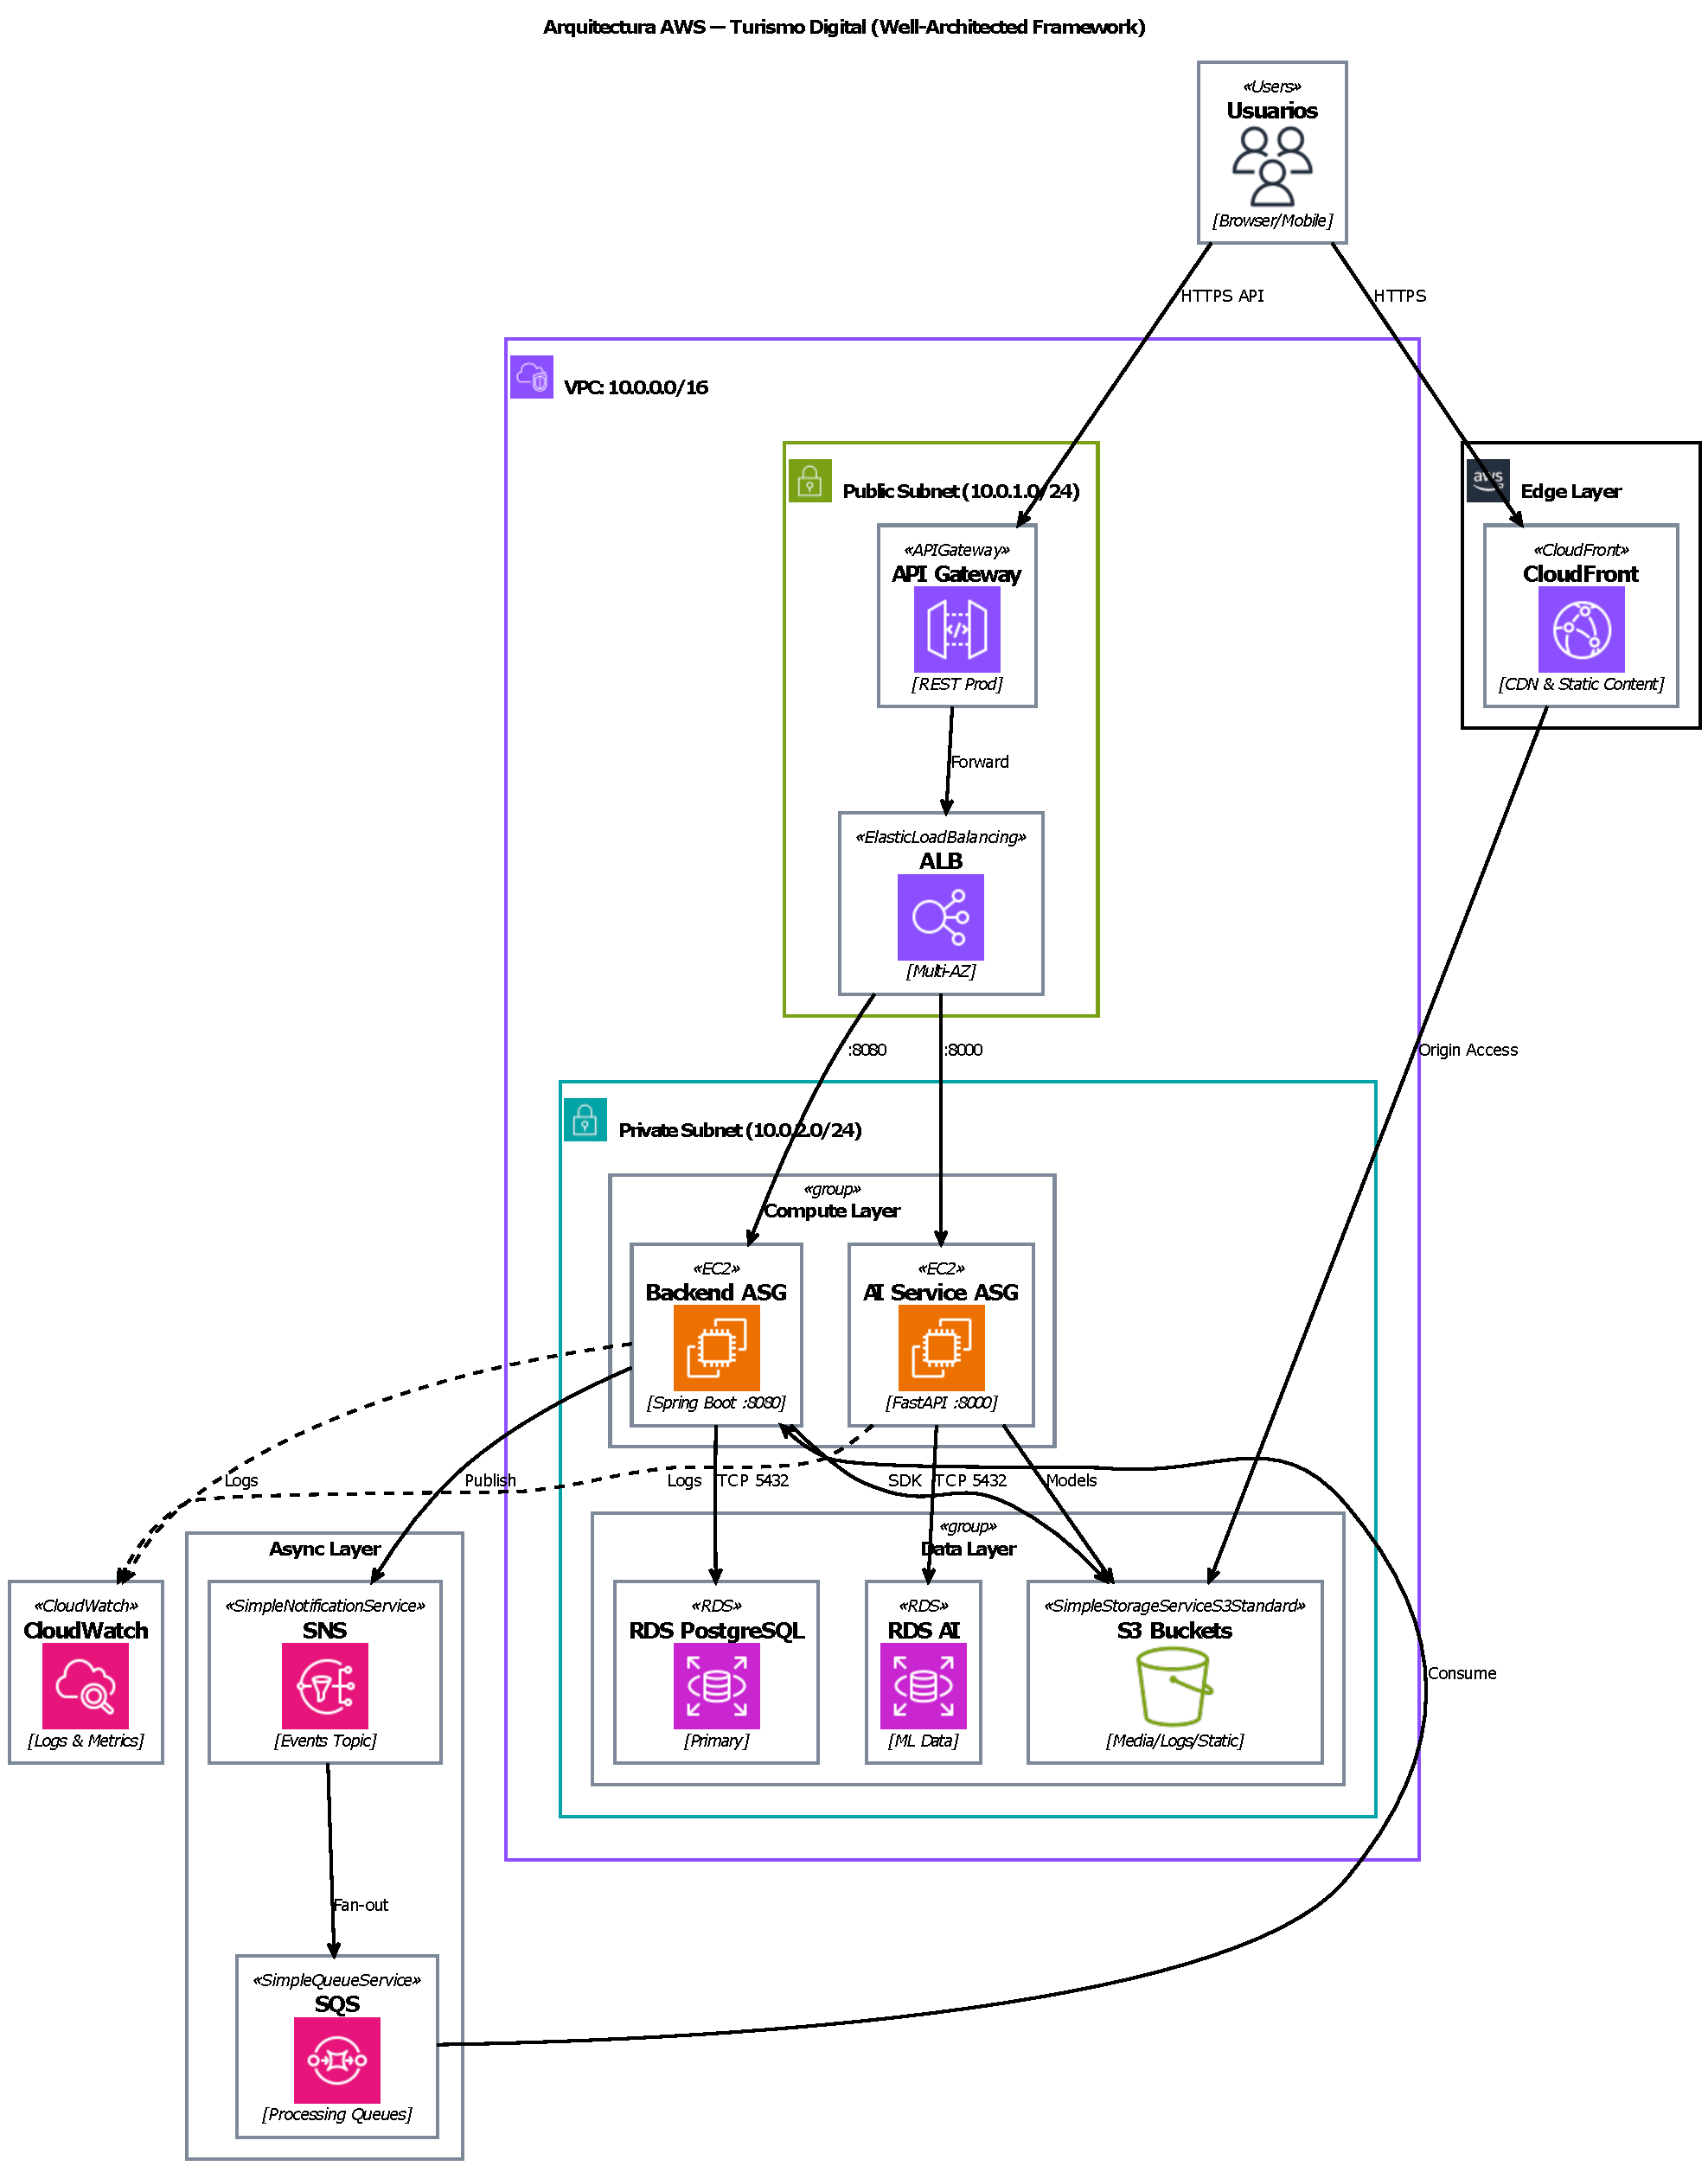
\includegraphics[width=0.85\textwidth,height=0.7\textheight,keepaspectratio]{figures/uml.deployment.aws-services.pdf}
    \caption{Arquitectura cloud-native de referencia en AWS (alineada al repositorio de infraestructura)}
    \label{fig:arquitectura_aws}
\end{figure}

\subsection*{Justificación de AWS}

Se compararon diferentes proveedores de nube:

\begin{table}[h]
\centering
\textbf{Tabla 1}

\textit{Comparación de proveedores de servicios en la nube}

\begin{tabular}{l p{4cm} p{4cm}}
\hline
Proveedor & Ventajas & Limitaciones \\
\hline
AWS & Madurez, elasticidad, servicios IA & Complejidad inicial \\
Azure & Integración Microsoft & Dependencia del ecosistema \\
GCP & BigQuery potente & Menor presencia regional \\
\hline
\end{tabular}
\end{table}

AWS fue seleccionado por: autoescalamiento y alta disponibilidad (SLA 99.99\%); ecosistema maduro de microservicios y servicios de IA integrados; reducción de carga operativa mediante servicios administrados.

\subsection*{Vista de componentes y correspondencia tecnológica}

La Tabla~\ref{tab:componentes} resume la correspondencia entre capas lógicas, tecnologías en los repositorios de aplicación e infraestructura y recursos AWS documentados.

\begin{table}[h]
\centering
\textbf{Tabla 2}
\caption{Vista de componentes (repositorios de código e infraestructura)}
\label{tab:componentes}
\small
\begin{tabular}{p{2.6cm} p{3.2cm} p{4.2cm} p{3.8cm}}
\hline
Rol & Tecnología documentada & Propósito & Recursos AWS asociados \\
\hline
Cliente web & React (Vite) & Interfaz de gestión y planificación & S3 + CloudFront \\
Cliente móvil & Android (Kotlin, Jetpack Compose) & Experiencia nativa & Publicación en tienda (fuera del aprovisionamiento S3) \\
Núcleo backend & Java 17, Spring Boot & API REST, reglas de negocio, JWT & EC2 detrás de ALB (p.\,ej.\ puerto 8080) \\
Servicio IA & Python 3.x, FastAPI & Recomendación, compatibilidad, ML (p.\,ej.\ Scikit-learn) & EC2 detrás de ALB (p.\,ej.\ puerto 8000) \\
Entrada API & API Gateway REST & Punto único de entrada, enrutamiento & API Gateway \\
Balanceo & Application Load Balancer & Distribución y health checks & ALB \\
Persistencia & PostgreSQL 15.4 & Datos relacionales & RDS (db.t3.micro) \\
Objetos & --- & Medios, \textit{frontend} estático & S3 \\
Eventos & --- & Desacoplamiento asíncrono & SNS, SQS \\
Observabilidad & --- & Logs y métricas & CloudWatch \\
\hline
\end{tabular}
\end{table}

\subsection*{Arquitectura cloud-native implementada}

La solución implementa una arquitectura escalable basada en servicios gestionados de AWS optimizados para entornos Academy:

\begin{itemize}
\item \textbf{Capa de exposición:} Amazon API Gateway (APIs REST) con políticas de limitación de tasa documentadas; Application Load Balancer para distribución de tráfico entre grupos de instancias; Amazon CloudFront como CDN frente al bucket S3 del cliente web React.
\item \textbf{Capa de computación:} Instancias EC2 \texttt{t3.micro} con Auto Scaling Groups para el núcleo backend (Spring Boot) y el microservicio de IA (FastAPI).
\item \textbf{Capa de datos:} Amazon RDS para PostgreSQL 15.4 en clase \texttt{db.t3.micro} para persistencia transaccional y analítica ligera; Amazon S3 para almacenamiento de medios y artefactos; bases de datos lógicas separables para dominio operativo del backend y del servicio de IA según la configuración documentada en infraestructura.
\item \textbf{Mensajería:} Amazon SQS para colas de eventos asíncronos; Amazon SNS para publicación de eventos (p.\,ej.\ eventos de usuario y de recomendación, según variables de entorno documentadas).
\item \textbf{Monitoreo:} Amazon CloudWatch para logs, métricas y alarmas; health checks asociados al balanceador y a los grupos de autoescalado.
\end{itemize}

\subsection*{Flujo de datos y procesamiento}

\begin{enumerate}
\item El navegador obtiene el cliente web React desde Amazon S3 a través de Amazon CloudFront; el cliente móvil Android invoca las mismas APIs HTTPS.
\item Las solicitudes API atraviesan Amazon API Gateway hacia el Application Load Balancer.
\item El balanceador distribuye tráfico entre instancias EC2 del backend Spring Boot y del microservicio FastAPI.
\item Los eventos de dominio se publican en tópicos SNS y se consumen mediante colas SQS (patrón publicación/suscripción y colas documentado en infraestructura).
\item Tanto el backend como el servicio de IA acceden a Amazon RDS (PostgreSQL) y a Amazon S3 según sus responsabilidades.
\item Amazon CloudWatch centraliza registros y métricas de API Gateway, ALB y servicios de cómputo para operación y alarmas.
\end{enumerate}

\subsection*{Motor de Recomendaciones y Matching Social}

El sistema implementa un modelo híbrido de recomendación:

\begin{equation}
\hat{r}_{ui} = \alpha f_{collab}(u,i) + (1-\alpha) f_{content}(u,i)
\end{equation}

donde $f_{collab}(u,i) = p_u^T q_i$. El microservicio de IA (FastAPI) ejecuta algoritmos de aprendizaje automático (p.\,ej.\ Scikit-learn) para compatibilidad entre viajeros y recomendaciones contextuales, desplegado en el grupo de autoescalado EC2 documentado detrás del mismo balanceador de aplicaciones.

\subsection*{Implementación en AWS Academy Learner Lab}

La arquitectura está dimensionada para el entorno AWS Academy Learner Lab, respetando restricciones documentadas en el repositorio de infraestructura (p.\,ej.\ tipos de instancia \texttt{t3.micro}, región acotada, perfiles IAM predeterminados del laboratorio, ausencia de NAT Gateway o IP elástica en el modo documentado, RDS single-AZ sin cifrado obligatorio en ese entorno acotado):

\begin{itemize}
\item \textbf{Infraestructura optimizada:} Instancias EC2 \texttt{t3.micro} con Auto Scaling Groups para backend y servicio de IA, con límites de capacidad propios del laboratorio.
\item \textbf{Base de datos:} Amazon RDS PostgreSQL 15.4 en clase \texttt{db.t3.micro}, con políticas de respaldo y almacenamiento acordes a la plantilla de despliegue.
\item \textbf{Almacenamiento:} Buckets S3 para \textit{frontend} estático, medios y registros, con políticas de ciclo de vida donde apliquen.
\item \textbf{Red:} VPC con subredes, grupos de seguridad segregados por servicio y listas de control de acceso a la red para evitar comunicaciones directas no deseadas entre servicios.
\item \textbf{Monitoreo:} CloudWatch con retención de logs acotada (p.\,ej.\ 14 días documentados) y alarmas sobre umbrales de CPU y rendimiento.
\end{itemize}

La implementación académica garantiza: \textbf{(i)} viabilidad bajo restricciones del laboratorio; \textbf{(ii)} trazabilidad de la topología mediante scripts de aprovisionamiento; \textbf{(iii)} base para endurecimiento y migración a producción (cifrado avanzado, alta disponibilidad multi-AZ, identidad federada) cuando el contexto lo permita; \textbf{(iv)} costos acotados para entorno educativo.

\subsection*{Roadmap de Transformación Digital}

La implementación sigue una estrategia de transformación digital incremental con entregas de valor continuas:

\textbf{Fase 1 - MVP Empresarial:} Desarrollo del núcleo transaccional con integración de proveedores clave, procesamiento de pagos y funcionalidades básicas de reservas.

\textbf{Fase 2 - Inteligencia de Negocio:} Implementación del motor de recomendaciones híbrido, analytics básicos y dashboards para operadores turísticos.

\textbf{Fase 3 - Ecosistema Colaborativo:} Incorporación de funcionalidades de matching social, formación de grupos y marketplace de experiencias compartidas.

\textbf{Fase 4 - Optimización Avanzada:} Implementación de modelos predictivos para gestión de estacionalidad, pricing dinámico y optimización de recursos.

\textbf{Fase 5 - Escalabilidad Global:} Expansión a nuevos mercados, integración con sistemas legacy de grandes operadores y certificaciones de seguridad empresarial.

Se adopta metodología DevOps con CI/CD automatizado para garantizar calidad y velocidad de entrega.

\subsection*{Ventaja Competitiva Estratégica}

La solución se diferencia fundamentalmente de las plataformas basadas en IA generativa conversacional:

\begin{itemize}
\item \textbf{Integración con procesos core:} La inteligencia artificial se integra directamente en los sistemas de gestión operativa, no solo en interfaces de usuario.
\item \textbf{Optimización matemática rigurosa:} Implementación de algoritmos formales para optimización de recursos y predicción de demanda.
\item \textbf{Eficiencia computacional:} Arquitectura optimizada para procesamiento a gran escala con costos predecibles.
\item \textbf{Ecosistema de valor de red:} Creación de efectos de red positivos mediante colaboración entre usuarios.
\item \textbf{Inteligencia de negocio integrada:} Analítica avanzada para toma de decisiones estratégicas de operadores.
\end{itemize}

\subsection*{Impacto Empresarial y Transformación del Sector}

La implementación de esta solución genera impacto transformador en múltiples dimensiones:

\textbf{Impacto Operativo:}
\begin{itemize}
\item Reducción del 30-40\% en costos operativos mediante automatización y optimización de recursos.
\item Mejora del 25\% en ocupación promedio mediante gestión inteligente de estacionalidad.
\item Incremento del 20\% en eficiencia de conversión mediante personalización contextual.
\end{itemize}

\textbf{Impacto Estratégico:}
\begin{itemize}
\item Creación de nuevas fuentes de ingresos mediante marketplace de servicios colaborativos.
\item Diferenciación competitiva sostenible mediante efectos de red y lealtad de comunidad.
\item Inteligencia de negocio avanzada para toma de decisiones estratégicas.
\end{itemize}

\textbf{Impacto Social:}
\begin{itemize}
\item Democratización del acceso a experiencias turísticas personalizadas.
\item Facilitación de viajes colaborativos que reducen costos individuales.
\item Creación de comunidades que fomentan el turismo sostenible y consciente.
\end{itemize}

La solución representa una verdadera transformación digital que reestructura la cadena de valor del turismo y posiciona a Colombia como líder en innovación turística tecnológica.

\subsection*{Optimización de capacidad}

La planificación de recursos turísticos se modela mediante programación lineal:

\begin{equation}
\text{Maximizar } \sum_{i=1}^{n} x_i R_i \quad \text{sujeto a } \sum_{i=1}^{n} x_i C_i \leq \text{Capacidad}
\end{equation}

La predicción de demanda utiliza modelos SARIMA para anticipar picos y ajustar recomendaciones adaptativas.

%================================================================================
\section{Arquitectura Empresarial}
%================================================================================

La solución se estructura con un enfoque de arquitectura empresarial por capas, alineando capacidades de negocio con componentes técnicos desplegables. Esta vista integra decisiones funcionales, de datos y de plataforma con criterios de escalabilidad y operación continua.

\subsection{Capa de Negocio}

En la capa de negocio se identifican capacidades principales: gestión de identidad del viajero, planificación de viajes, coordinación social, recomendación inteligente y analítica operativa. Estas capacidades se materializan en flujos de valor donde el usuario crea intención de viaje, establece conexiones y ejecuta itinerarios con apoyo de recomendación contextual.

\subsection{Capa de Aplicación}

La capa de aplicación se compone de cuatro contenedores principales: cliente web (React/Vite), cliente móvil (Android/Kotlin), backend transaccional (Spring Boot) y microservicio de IA (FastAPI). El backend concentra reglas de dominio, autenticación JWT y exposición de APIs de usuario, viaje y funciones sociales. El servicio de IA encapsula modelos de recomendación, perfilamiento y \textit{matching}, desacoplado del núcleo transaccional para facilitar evolución algorítmica independiente.

\subsection{Capa de Datos}

La capa de datos combina persistencia relacional y almacenamiento de objetos. El dominio transaccional se apoya en entidades relacionales (\textit{users}, \textit{travel\_plans}, \textit{travel\_plan\_activities}, \textit{reservations}), mientras la capa de objetos en S3 soporta activos estáticos, medios y artefactos de soporte. La integración asíncrona mediante SNS/SQS habilita desacoplamiento temporal para eventos de usuario y recomendación, reduciendo acoplamiento entre productores y consumidores.

\subsection{Capa Tecnológica}

La capa tecnológica está definida por la infraestructura versionada: API Gateway, Application Load Balancer, Auto Scaling Groups sobre EC2 \texttt{t3.micro}, RDS PostgreSQL \texttt{db.t3.micro}, S3, SNS, SQS y CloudWatch dentro de una VPC con subredes públicas e Internet Gateway en \texttt{us-east-1}. Esta composición materializa la plataforma como sistema distribuido cloud-native, con separación de responsabilidades por servicio y observabilidad centralizada.

\subsection{Alineación estratégica de transformación digital}

La arquitectura empresarial conecta la estrategia de transformación digital con resultados operacionales verificables: automatización de procesos, personalización a escala, coordinación social y soporte a decisiones basadas en datos. La separación entre capacidades de negocio y unidades de despliegue permite trazar inversión tecnológica hacia indicadores de eficiencia, experiencia y resiliencia operativa.

%================================================================================
\section{Gobernanza de Arquitectura}
%================================================================================

La gobernanza se concibe como un sistema de control técnico y operativo que combina estándares de diseño, controles automáticos en CI/CD y supervisión en tiempo de ejecución.

\subsection{Modelo de gobernanza técnica}

Se adopta un modelo federado por repositorios, donde cada dominio técnico (web, móvil, backend, IA, infraestructura) conserva autonomía de implementación dentro de lineamientos comunes: contratos API versionados, separación por capas, políticas de seguridad mínimas y convenciones de despliegue en AWS. Este esquema reduce dependencia de equipos y habilita evolución incremental controlada.

\subsection{Control de estándares arquitectónicos}

El control de estándares se materializa en: (i) convenciones de estructura por capas en backend y móvil; (ii) contratos HTTP explícitos en API Gateway y servicios; (iii) uso de componentes AWS definidos en scripts como fuente de verdad de despliegue; (iv) versionamiento de configuración operativa en \texttt{config.json}. La gobernanza de cambios privilegia trazabilidad de decisiones y reproducibilidad de infraestructura.

\subsection{CI/CD como mecanismo de enforcement}

Los flujos GitHub Actions en backend, IA, web y móvil aplican controles automáticos: escaneo de vulnerabilidades con Trivy, análisis estático con SonarCloud y etapas de construcción/artefactado por repositorio. Este mecanismo transforma la gobernanza en control ejecutable, al bloquear integración ante incumplimientos de seguridad o calidad definidos en pipeline.

\subsection{Observabilidad y control operacional}

CloudWatch centraliza logs y métricas de componentes perimetrales y de cómputo, con alarmas sobre CPU, profundidad de colas y estados de servicio. Los \textit{health checks} de ALB y la supervisión de ASG permiten detectar degradación y gatillar recuperación automática a nivel de instancia. Este ciclo observación--decisión--acción constituye el núcleo de gobernanza operacional en ambiente distribuido.

\subsection{Gestión de cambios arquitectónicos}

La gestión de cambios sigue una secuencia: propuesta de modificación, validación técnica en repositorio correspondiente, verificación de impacto en interfaces y datos, ejecución de pipeline y despliegue controlado. En contexto académico, la fase final incluye \textit{handoff} manual de despliegue; no obstante, los controles previos reducen riesgo de regresión funcional y de seguridad.

%================================================================================
\section{Atributos de Calidad Integrados en las Decisiones Arquitectónicas}
%================================================================================

Los atributos de calidad se incorporan como escenarios verificables que orientan decisiones de diseño y operación.

\subsection{Disponibilidad y escalabilidad}

La elección de ALB + ASG con límites \texttt{min/max/desired} por servicio responde a escenarios de falla de instancia y crecimiento de carga. La arquitectura privilegia recuperación por reemplazo de nodos y escalado horizontal dentro de restricciones de laboratorio (\texttt{t3.micro}, máximo de instancias), manteniendo continuidad funcional del plano API.

\subsection{Rendimiento y eficiencia}

La separación backend/IA evita contención de recursos entre transacciones y cómputo de recomendación. La mensajería SNS/SQS absorbe variabilidad temporal y desacopla procesos no estrictamente síncronos. Esta decisión mitiga picos de demanda y reduce latencia percibida en operaciones críticas del usuario.

\subsection{Seguridad y protección}

La seguridad se articula en capas: autenticación/autorización JWT a nivel de aplicación, control perimetral por API Gateway/ALB y segmentación por security groups para acceso a RDS. En ciclo de vida, Trivy y SonarCloud operan como controles de cadena de suministro, reforzando prevención temprana de vulnerabilidades.

\subsection{Mantenibilidad y evolución}

La modularidad por repositorios y por contenedores técnicos permite cambios localizados (p.\,ej.\ algoritmos en IA o ajustes de UX en web/móvil) con menor acoplamiento estructural. El versionamiento de infraestructura y pipelines uniformes facilita evolución gobernada sin perder coherencia sistémica.

\subsection{Interoperabilidad y compatibilidad}

El uso de APIs REST versionadas, DTOs y esquemas explícitos entre clientes y servicios responde a escenarios de interoperabilidad multi-cliente. Esta estrategia reduce fricción de integración y permite coexistencia de canales web y móvil sobre una misma base de capacidades.

\subsection{Observabilidad y operabilidad}

Los escenarios de calidad de detección temprana de incidentes se cubren mediante métricas y alarmas en CloudWatch, junto con endpoints de salud para backend e IA. La arquitectura convierte la observabilidad en capacidad transversal, imprescindible para gobernar un sistema distribuido con componentes autónomos.

%================================================================================
\section{Trazabilidad con Diagramas Arquitectónicos e Infraestructura}
%================================================================================

La consistencia del diseño se verifica mediante trazabilidad cruzada entre vistas arquitectónicas:

\begin{itemize}
\item \textbf{Diagramas C4 (contexto, contenedores, componentes):} sustentan la separación por capacidades y responsabilidades entre clientes, backend, servicio IA e integraciones de plataforma.
\item \textbf{Diagramas UML (componentes, despliegue, contexto, actividades, casos de uso):} detallan contratos técnicos, relaciones entre artefactos y comportamiento de flujos principales.
\item \textbf{Diagramas AWS y topología de red:} reflejan la implementación concreta definida en \texttt{voyager-infrastructure} (VPC, subredes, balanceo, cómputo, datos, mensajería, monitoreo).
\item \textbf{Diagrama CI/CD:} evidencia el modelo de gobernanza ejecutable, con controles automáticos de seguridad y calidad por repositorio.
\item \textbf{Diagrama ER físico:} conecta decisiones de dominio transaccional con persistencia relacional y políticas de acceso en red.
\end{itemize}

Esta trazabilidad garantiza que la arquitectura empresarial no permanezca como abstracción documental, sino como sistema verificable en artefactos de código, infraestructura y operación.

%================================================================================
\section{Seguridad del Sistema}
%================================================================================

La solución opera en un entorno distribuido con datos personales y transacciones; la seguridad se aborda de forma coherente con lo documentado en el repositorio de infraestructura y con las decisiones de aplicación descritas en la documentación técnica del proyecto (p.\,ej.\ JWT en el núcleo Spring Boot). No se declaran aquí componentes AWS que no figuren en dicho despliegue de referencia (p.\,ej.\ Cognito, WAF, DynamoDB, Redshift, X-Ray o Secrets Manager no constan en los scripts de infraestructura versionados).

\subsection{Cifrado en tránsito (TLS)}

Las comunicaciones externas hacia \textbf{Amazon API Gateway} y el \textbf{Application Load Balancer} utilizan HTTPS/TLS en el perímetro, conforme a la política de tráfico seguro descrita en infraestructura. \textit{Justificación:} reduce el riesgo de interceptación y manipulación en tránsito entre clientes web/móviles y el borde de la plataforma.

\subsection{Protección de datos en reposo}

\begin{itemize}
\item \textbf{Amazon RDS:} contraseñas robustas y acceso restringido por grupos de seguridad; en el modo Academy documentado puede aplicarse configuración single-AZ sin cifrado obligatorio, por lo que el endurecimiento con cifrado nativo de RDS debe planificarse explícitamente en despliegues productivos.
\item \textbf{Amazon S3:} buckets privados con cifrado de objetos según la política descrita en el repositorio de infraestructura (p.\,ej.\ SSE-S3 o equivalente documentado).
\end{itemize}

\textit{Justificación:} limita la exposición de datos ante compromiso de almacenamiento y refuerza el principio de defensa en profundidad al migrar a entornos productivos.

\subsection{Autenticación y autorización a nivel de aplicación}

\begin{itemize}
\item \textbf{Autenticación stateless con JWT} implementada en el núcleo Spring Boot, según la arquitectura técnica del repositorio de documentación (cliente web con Axios e interceptores; cliente móvil con Retrofit/OkHttp).
\item \textbf{AWS IAM} en el laboratorio con los roles y perfiles exigidos por AWS Academy (p.\,ej.\ LabRole, LabInstanceProfile), aplicando el menor privilegio posible dentro de las restricciones del entorno académico.
\end{itemize}

\subsection{Control de acceso a red y API}

\begin{itemize}
\item \textbf{API Gateway:} punto de entrada centralizado con limitación de tasa (\textit{throttling}) documentada.
\item \textbf{VPC:} grupos de seguridad segregados por servicio y listas de control de acceso a la red (NACLs) para evitar comunicaciones directas no deseadas entre servicios, según el modelo de red del repositorio de infraestructura.
\end{itemize}

\subsection{Observabilidad y buenas prácticas}

\begin{itemize}
\item \textbf{Amazon CloudWatch} para registros, métricas y alarmas sobre CPU, memoria y salud de los endpoints.
\item Separación lógica de entornos (desarrollo, laboratorio, producción futura) y gobierno de credenciales alineado a las prácticas del equipo (sin asumir servicios de secretos gestionados no desplegados en la referencia actual).
\end{itemize}

%================================================================================
\section{Metodología}
%================================================================================

La presente investigación propone el diseño metodológico para la construcción de un dataset propio orientado al sector turístico colombiano, con el objetivo de desarrollar y evaluar un sistema de recomendación contextual basado en una arquitectura cognitiva. Dado que actualmente no existen datasets públicos suficientemente adaptados al contexto colombiano, esta investigación plantea la creación estructurada de un dataset experimental. Al momento de este trabajo, el sistema no ha sido implementado en producción; por tanto, la metodología describe el diseño propuesto y el marco experimental previsto.

\subsection{Diseño del Dataset Propuesto}

El dataset se estructurará bajo un enfoque \textit{data-centric}. Se contemplan tres fuentes: datos transaccionales (reservas, cancelaciones, precios dinámicos); datos de comportamiento in-app (navegación, búsquedas, clics, preferencias declaradas); variables contextuales externas (temporada, festividades, clima por región).

El modelo de datos se organiza en: \textbf{Nivel Usuario} (identificador anonimizado, preferencias, historial); \textbf{Nivel Transacción} (destino, fecha, precio, tipo de servicio); \textbf{Nivel Contextual} (región, temporada, indicadores de demanda).

\subsection{Mapeo a la Arquitectura Cognitiva}

El dataset se estructura para alimentar los tres componentes cognitivos: \textbf{Memoria Episódica} integra secuencias temporales (historial de reservas, navegación, respuestas promocionales, historial de interacción social: grupos formados, solicitudes enviadas/recibidas), modeladas mediante embeddings secuenciales. \textbf{Memoria Semántica} contiene taxonomías de destinos, segmentaciones por tipo de viajero, relaciones estacionalidad-comportamiento y perfiles de afinidad para \textit{matching} social, modelada mediante esquemas dimensionales y grafos semánticos. \textbf{Memoria Procedimental} incorpora reglas (incentivos en temporada baja, priorización de regiones con menor ocupación, ajuste dinámico de recomendaciones, criterios de emparejamiento para viajes colaborativos), implementadas como funciones parametrizables.

\subsection{Gobernanza y Preparación de Datos}

Anonimización y pseudonimización; normalización de categorías; validación de consistencia temporal; detección de valores atípicos en precios. Almacenamiento conceptual: Data Lake para datos crudos y modelo dimensional para análisis estructurado.

\subsection{Diseño Experimental}

División en entrenamiento (70\%), validación (15\%) y prueba (15\%); validación cruzada; comparación frente a baseline basado en popularidad global. El modelo híbrido se define como $\hat{r}_{ui} = \alpha f_{collab}(u,i) + (1-\alpha) f_{content}(u,i)$, donde $f_{collab}(u,i)$ y $f_{content}(u,i)$ son las estimaciones colaborativa y basada en contenido, y $\alpha \in [0,1]$ se estima experimentalmente.

\subsection{Métricas de Evaluación}

\textbf{Nivel Predictivo:} RMSE, MAE, Precision@K, Recall@K. \textbf{Nivel Territorial:} variación proyectada en distribución regional; sensibilidad ante cambios estacionales. \textbf{Nivel Experimental:} pruebas de significancia estadística con $\alpha = 0.05$ para la hipótesis $H_0: \mu_{modelo} = \mu_{baseline}$.

%================================================================================
\section{Evaluación}
%================================================================================

\subsection{Métricas propuestas}

La evaluación del sistema se plantea a través de métricas cuantitativas y cualitativas: precisión del sistema de recomendación (Precision@10); error de predicción (RMSE frente a baseline); impacto en estacionalidad de la demanda; tiempo promedio de planificación de viajes; tasa de retención de usuarios; nivel de interacción comunitaria; ROI estimado. Se aplicarán pruebas de significancia estadística para determinar si las diferencias frente a métodos tradicionales resultan relevantes.

\subsection{Discusión cualitativa}

En un contexto de crecimiento sostenido del turismo, la incorporación de inteligencia artificial y funcionalidades sociales podría representar una ventaja estratégica. La dimensión de viaje colaborativo y conexión entre usuarios aporta un diferencial de producto que las plataformas tradicionales no ofrecen, con potencial para mejorar retención, \textit{engagement} y satisfacción mediante la formación de comunidades de viajeros. Desde una perspectiva arquitectónica: establece separación clara de responsabilidades; mejora trazabilidad de procesos; facilita escalabilidad modular para incorporar nuevos servicios, incluyendo la capa social como componente extensible.

\subsection{Limitaciones del sistema}

\begin{itemize}
\item Dependencia de la calidad y disponibilidad de los datos de entrada; sin datos representativos del turismo colombiano, los modelos pueden sufrir sesgos.
\item Complejidad inicial en el modelado y parametrización del sistema; la calibración de $\alpha$ y de los modelos SARIMA requiere iteración.
\item Necesidad de validación empírica en entornos reales para confirmar efectividad; el diseño actual es conceptual y no ha sido desplegado en producción.
\end{itemize}

\subsection{Problemas prácticos}

\begin{itemize}
\item \textbf{Energía y costos:} La infraestructura AWS implica costos variables; en regiones con tráfico bajo, el modelo de pago por uso puede ser favorable, pero picos estacionales pueden incrementar facturación.
\item \textbf{Datos:} La construcción del dataset experimental depende de acuerdos con proveedores turísticos o de simulación; los datos sintéticos pueden no reflejar la realidad.
\item \textbf{Capacidad y latencia:} La inferencia en tiempo real depende del dimensionamiento de los grupos de autoescalado EC2 \texttt{t3.micro} y del Application Load Balancer; subdimensionar puede generar latencias elevadas o pérdida de solicitudes bajo picos de demanda.
\end{itemize}

\subsection{Consideraciones técnicas}

\begin{itemize}
\item La integración con sistemas externos (proveedores de vuelos, hoteles) depende de APIs heterogéneas; la estabilidad y el formato de los datos varían entre proveedores.
\item Los pipelines de integración continua y las imágenes de contenedor empleadas en desarrollo deben someterse a controles de seguridad de cadena de suministro (tema relacionado con la línea de trabajo de escaneo de imágenes y DevSecOps en la documentación de fundamentos de seguridad del repositorio).
\end{itemize}

%================================================================================
\section{Diagramas de Arquitectura (C4 Model)}
%================================================================================

Los diagramas C4 ilustran el sistema como conjunto de contenedores y relaciones; deben interpretarse de manera consistente con la topología del repositorio de infraestructura: clientes web y móvil, API Gateway, balanceador de aplicaciones, dos servicios de cómputo (Spring Boot y FastAPI), RDS PostgreSQL, S3, SNS/SQS y CloudFront/CloudWatch según corresponda.

\begin{figure}[H]
    \centering
    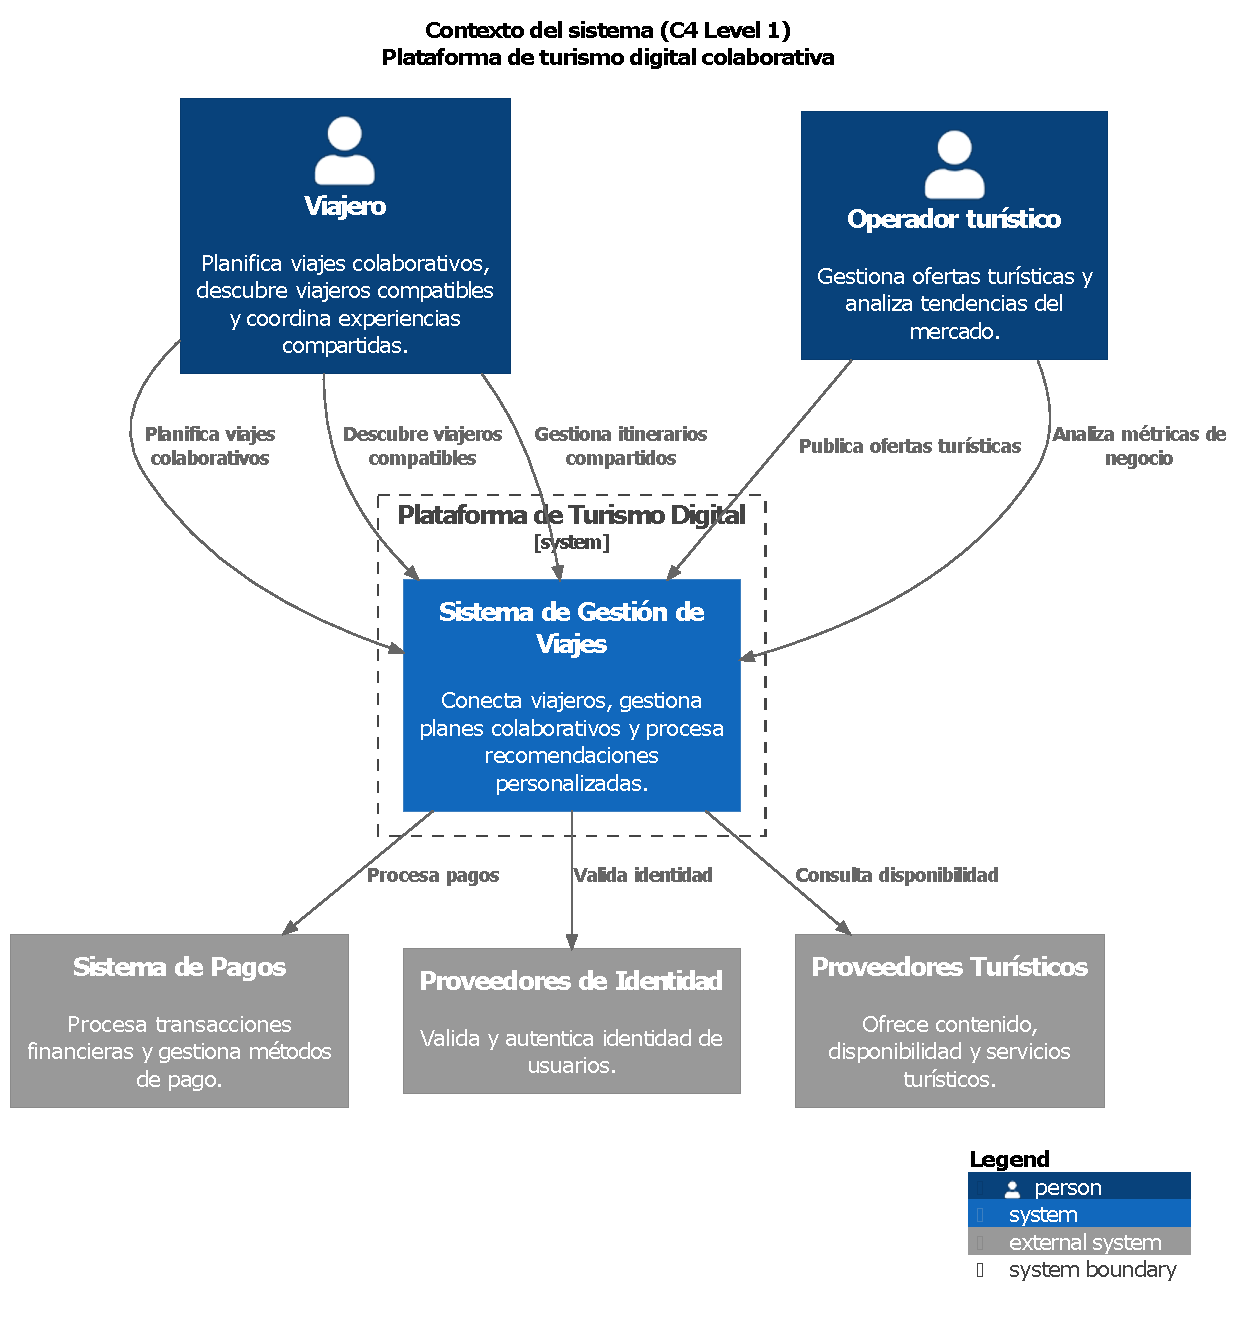
\includegraphics[width=0.85\textwidth,height=0.6\textheight,keepaspectratio]{figures/c4-model.level-1-context.pdf}
    \caption{Diagrama de contexto C4 (alineación con API Gateway, ALB y servicios de cómputo documentados)}
    \label{fig:contexto_c4}
\end{figure}

\begin{figure}[H]
    \centering
    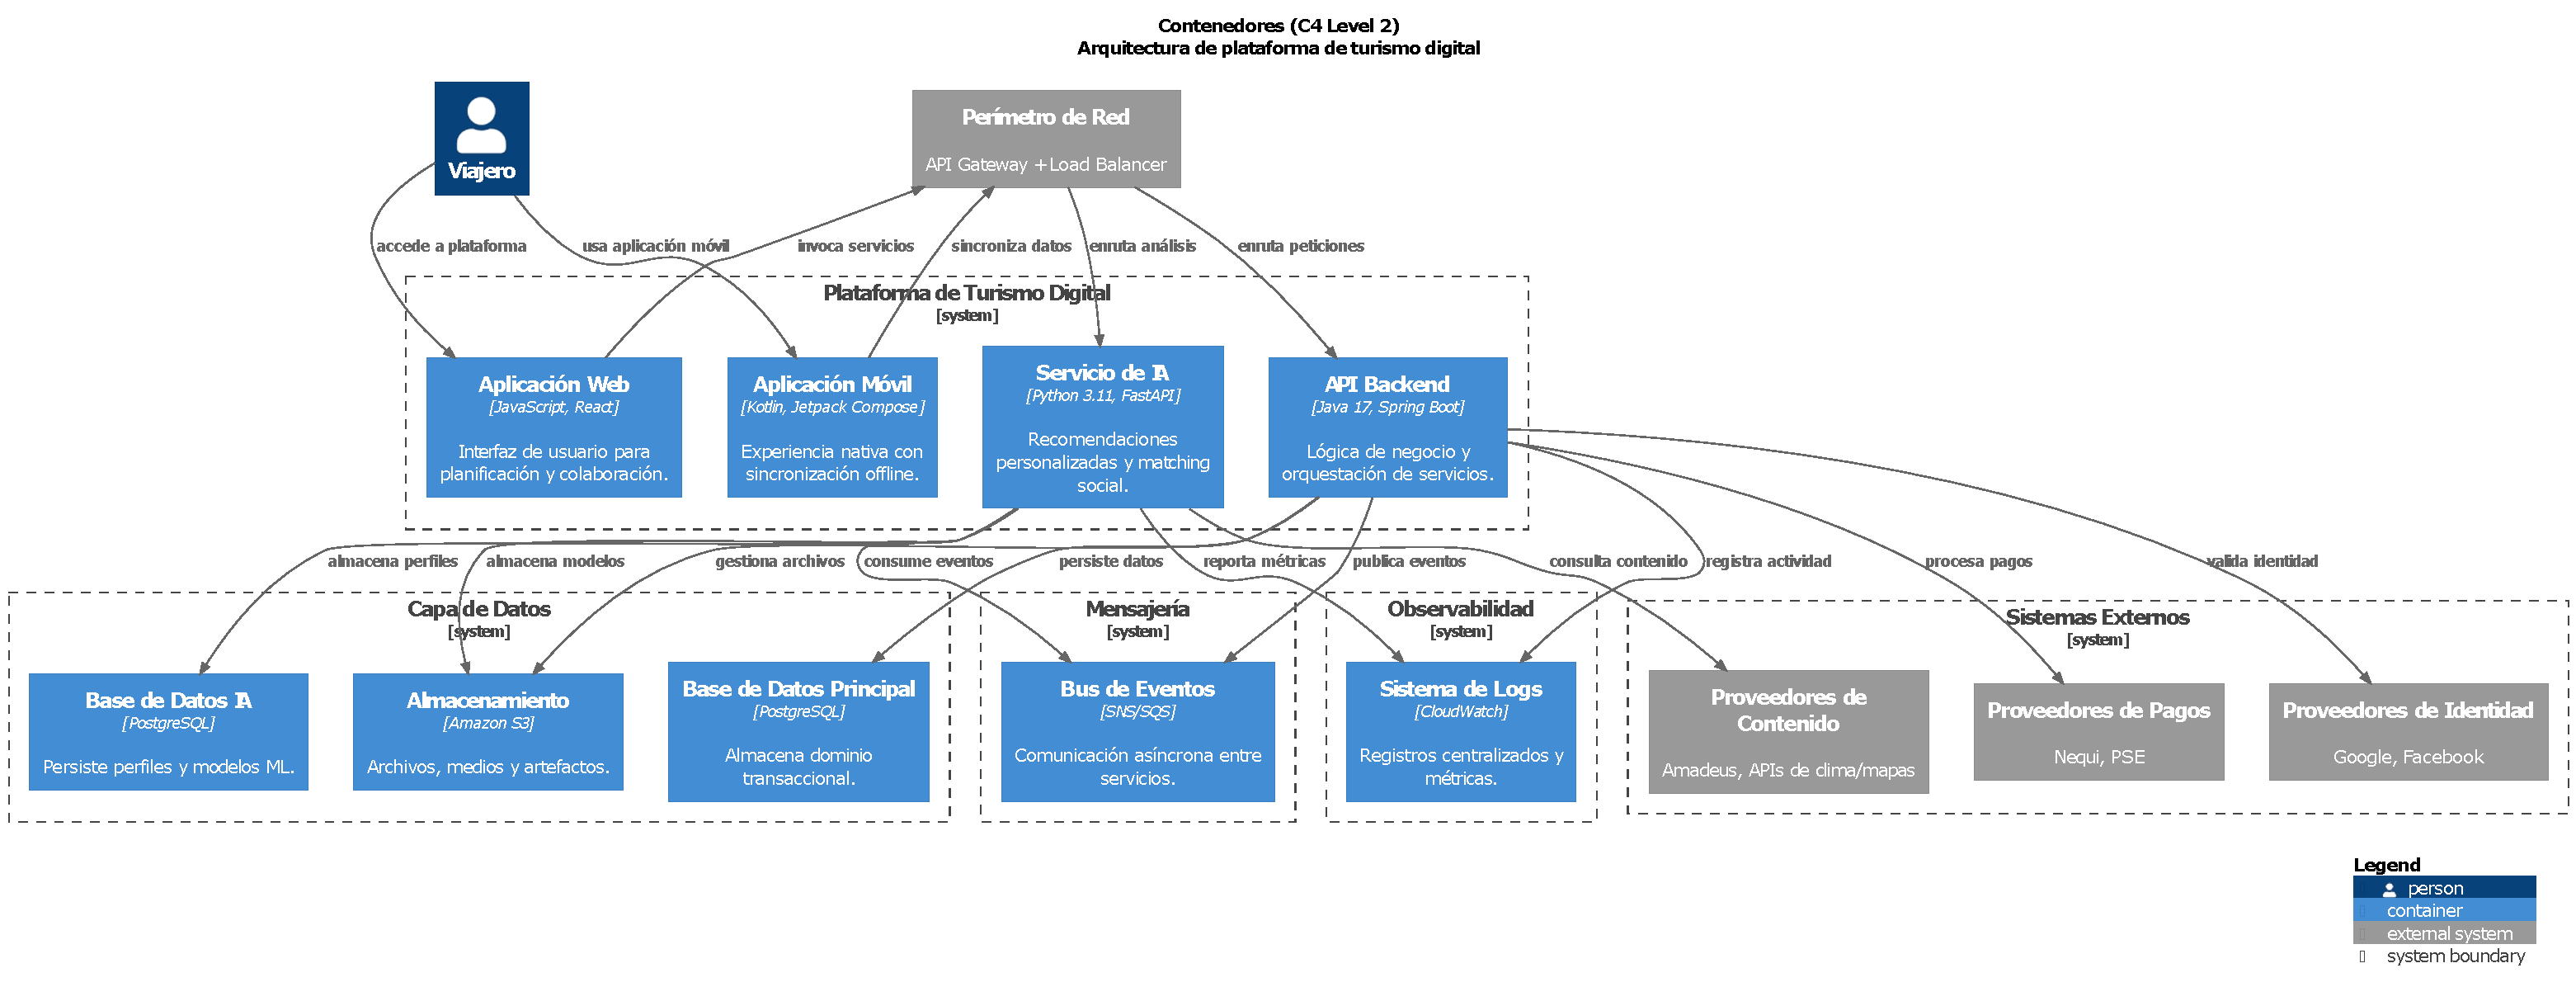
\includegraphics[width=0.85\textwidth,height=0.6\textheight,keepaspectratio]{figures/c4-model.level-2-containers.pdf}
    \caption{Diagrama de contenedores C4 (núcleo backend, microservicio IA, persistencia y mensajería)}
    \label{fig:contenedores_c4}
\end{figure}

\begin{figure}[H]
    \centering
    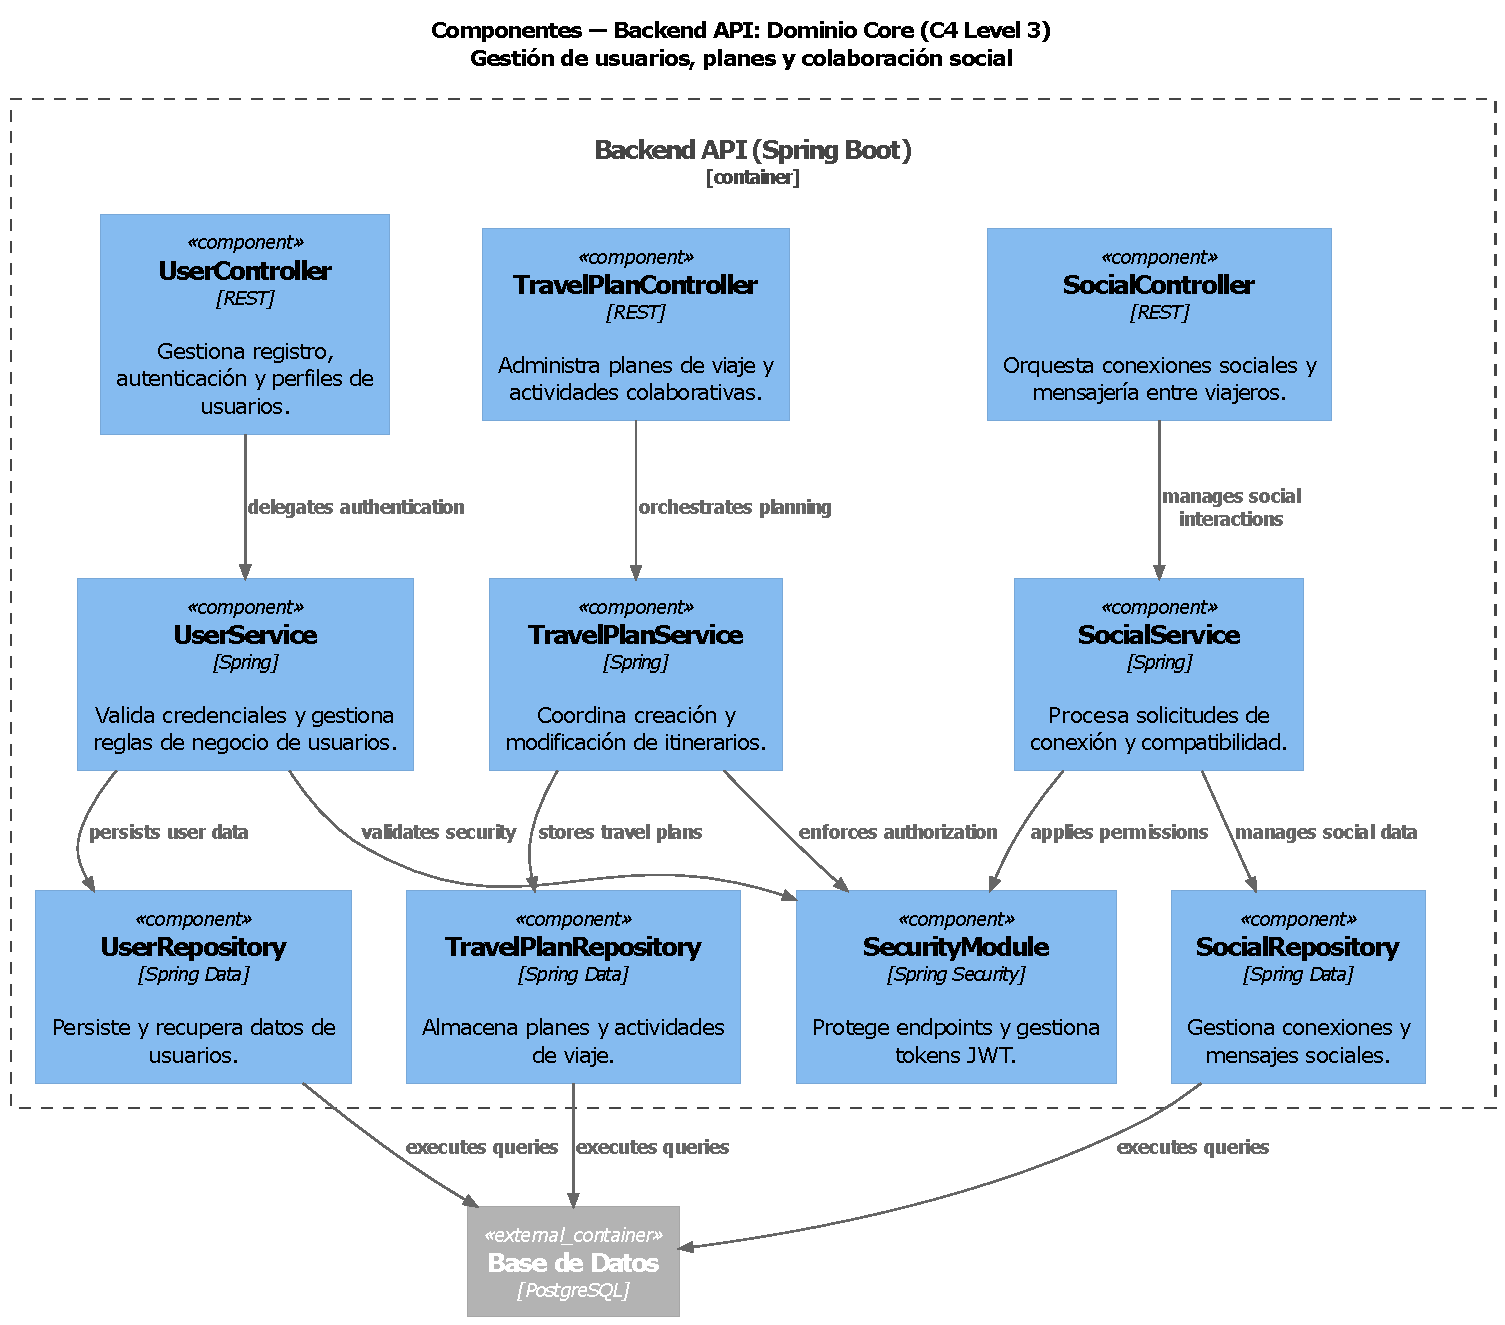
\includegraphics[width=0.85\textwidth,height=0.7\textheight,keepaspectratio]{figures/c4-model.level-3-components.backend.core.pdf}
    \caption{Diagrama de componentes del backend core (Spring Boot)}
    \label{fig:components_backend}
\end{figure}

\begin{figure}[H]
    \centering
    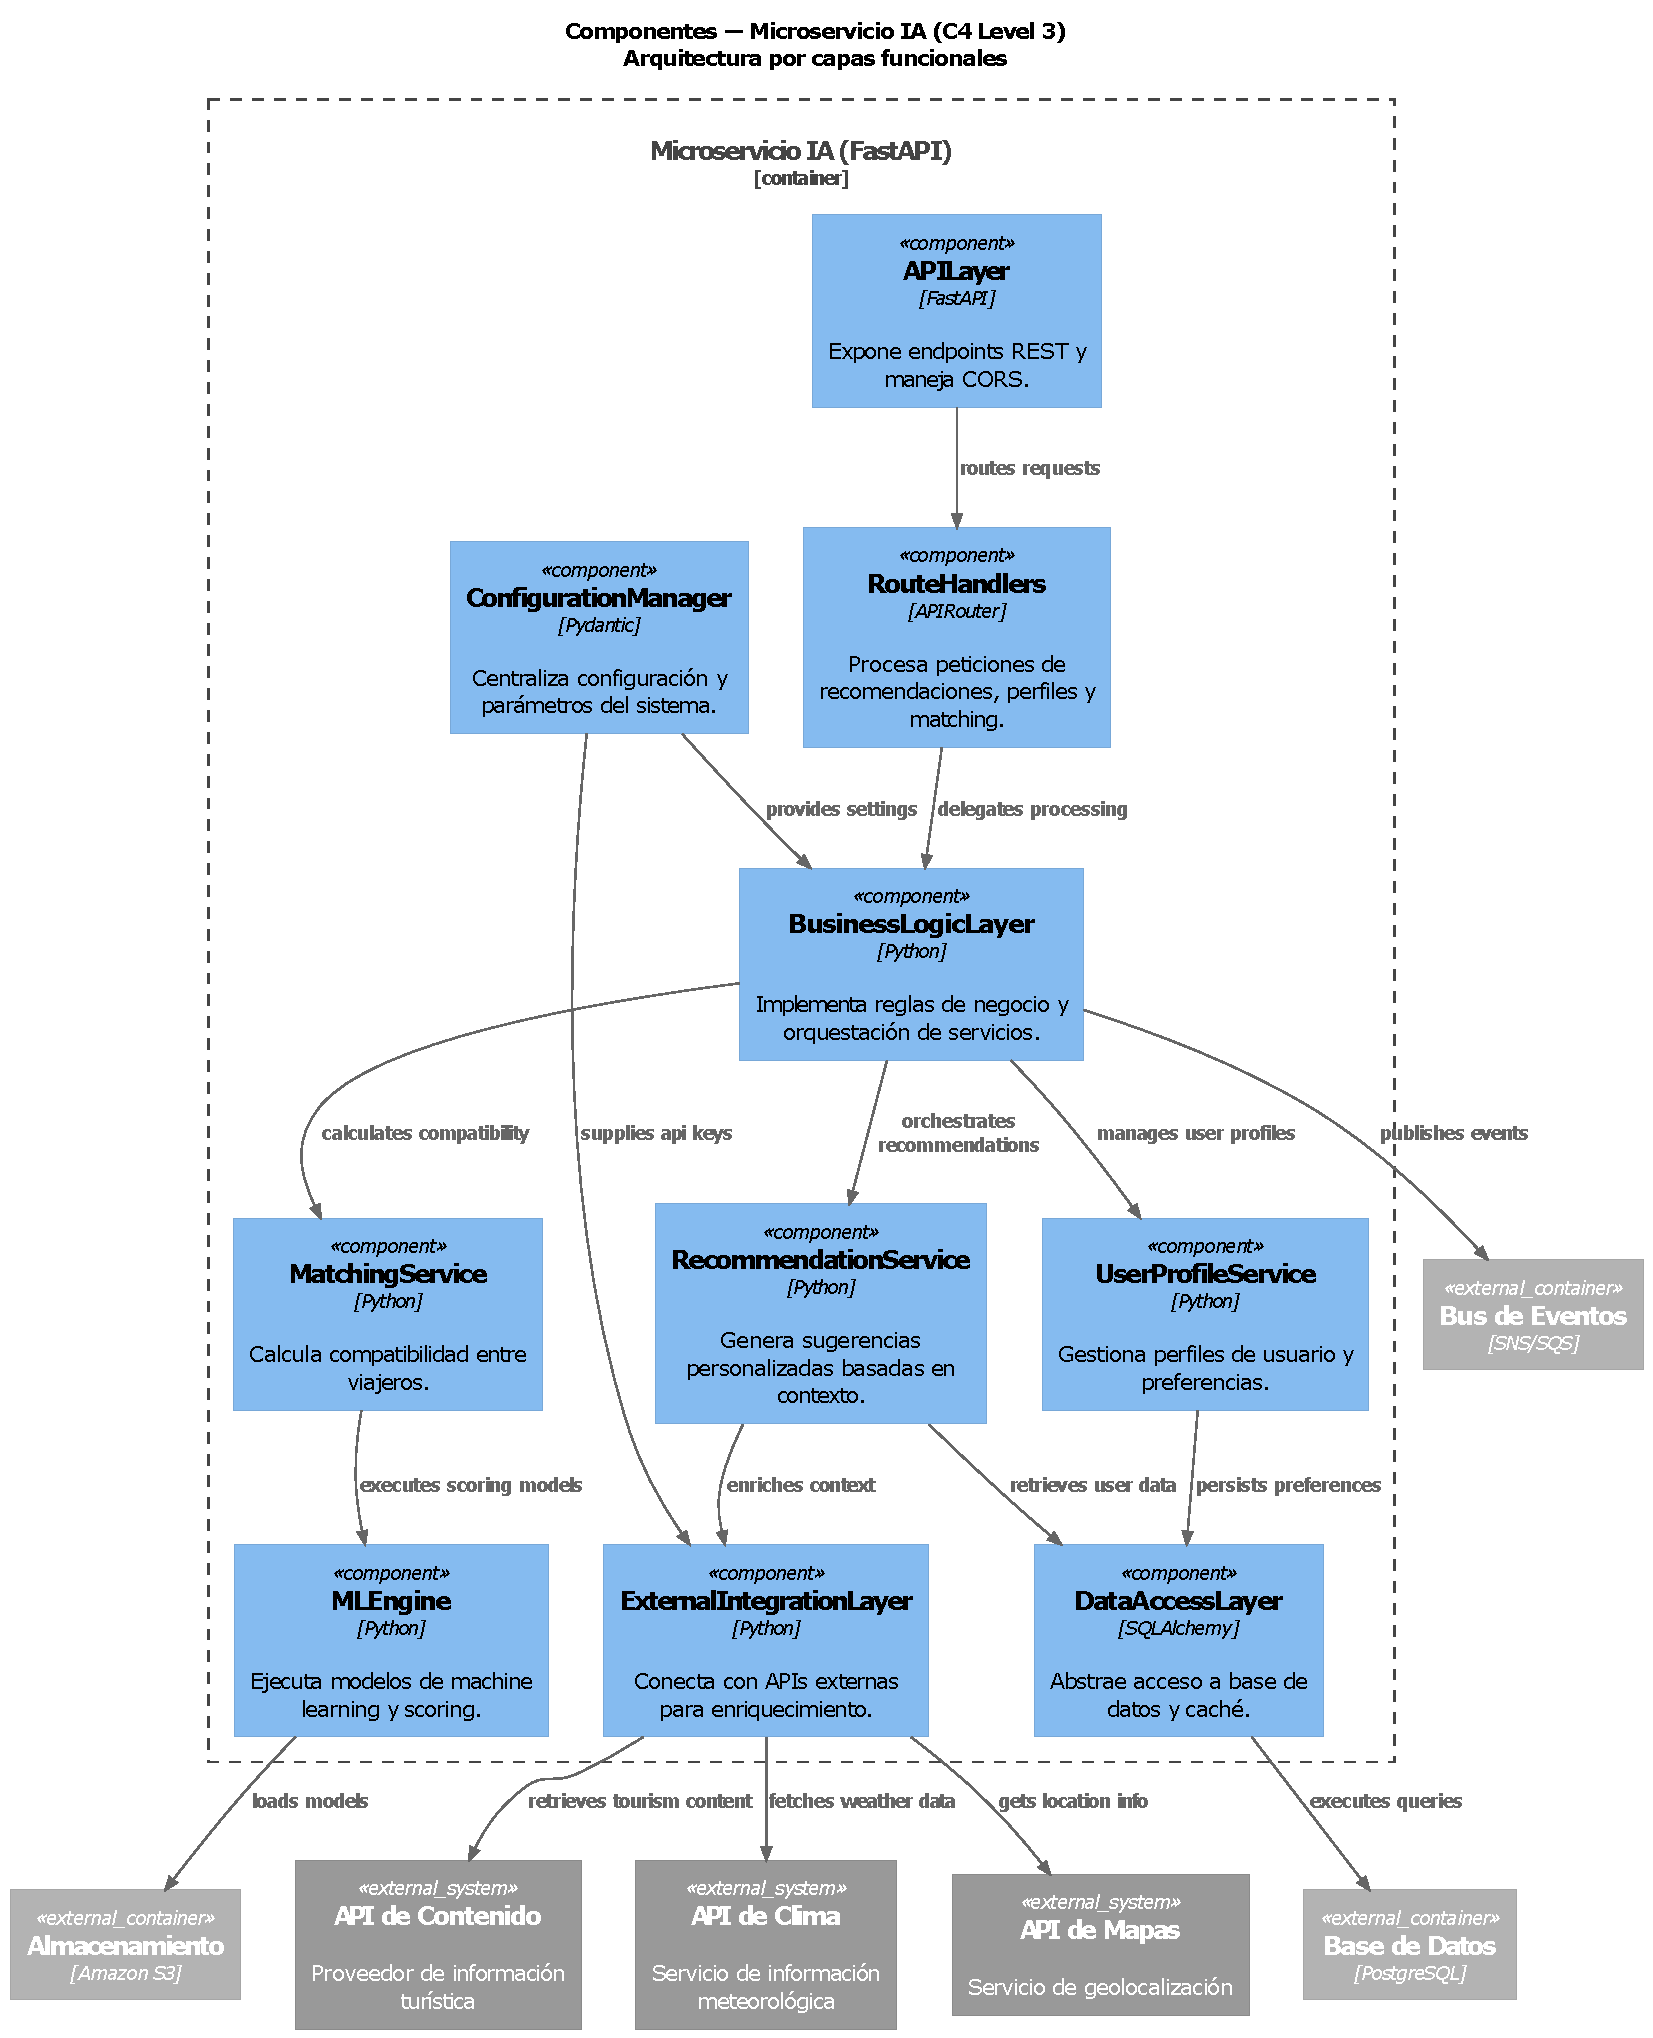
\includegraphics[width=0.85\textwidth,height=0.7\textheight,keepaspectratio]{figures/c4-model.level-3-components.ai-microservice.pdf}
    \caption{Diagrama de componentes del microservicio de IA (FastAPI)}
    \label{fig:components_ai}
\end{figure}

\begin{figure}[H]
    \centering
    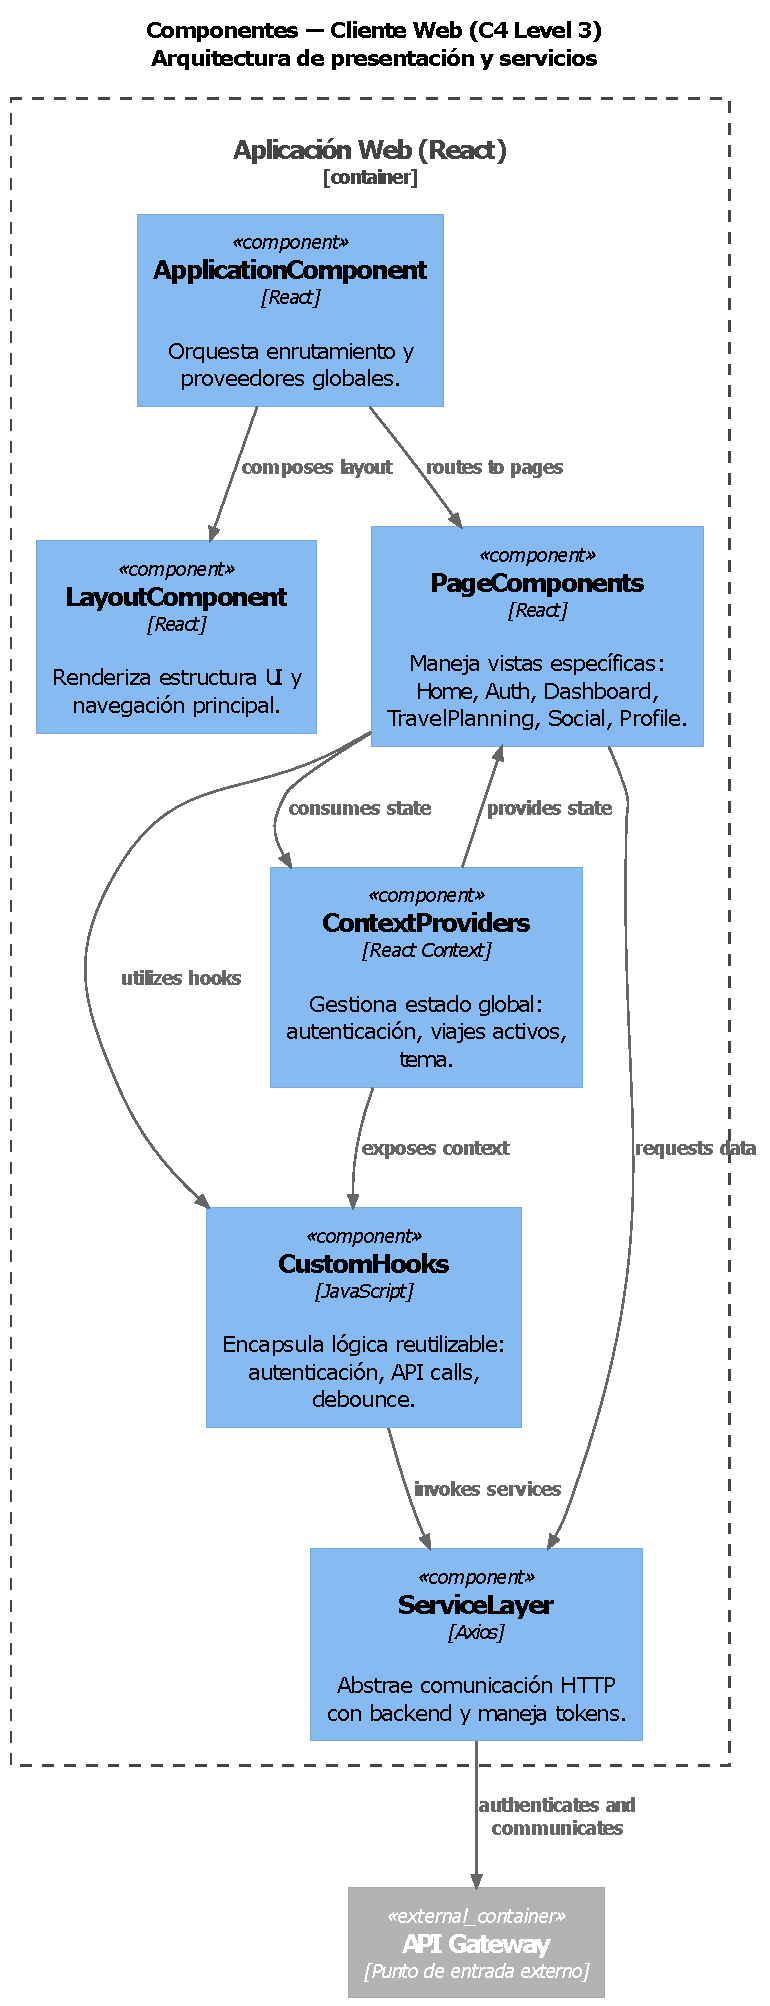
\includegraphics[width=0.85\textwidth,height=0.7\textheight,keepaspectratio]{figures/c4-model.level-3-components.web-client.pdf}
    \caption{Diagrama de componentes del cliente web (React)}
    \label{fig:components_web}
\end{figure}

\begin{figure}[H]
    \centering
    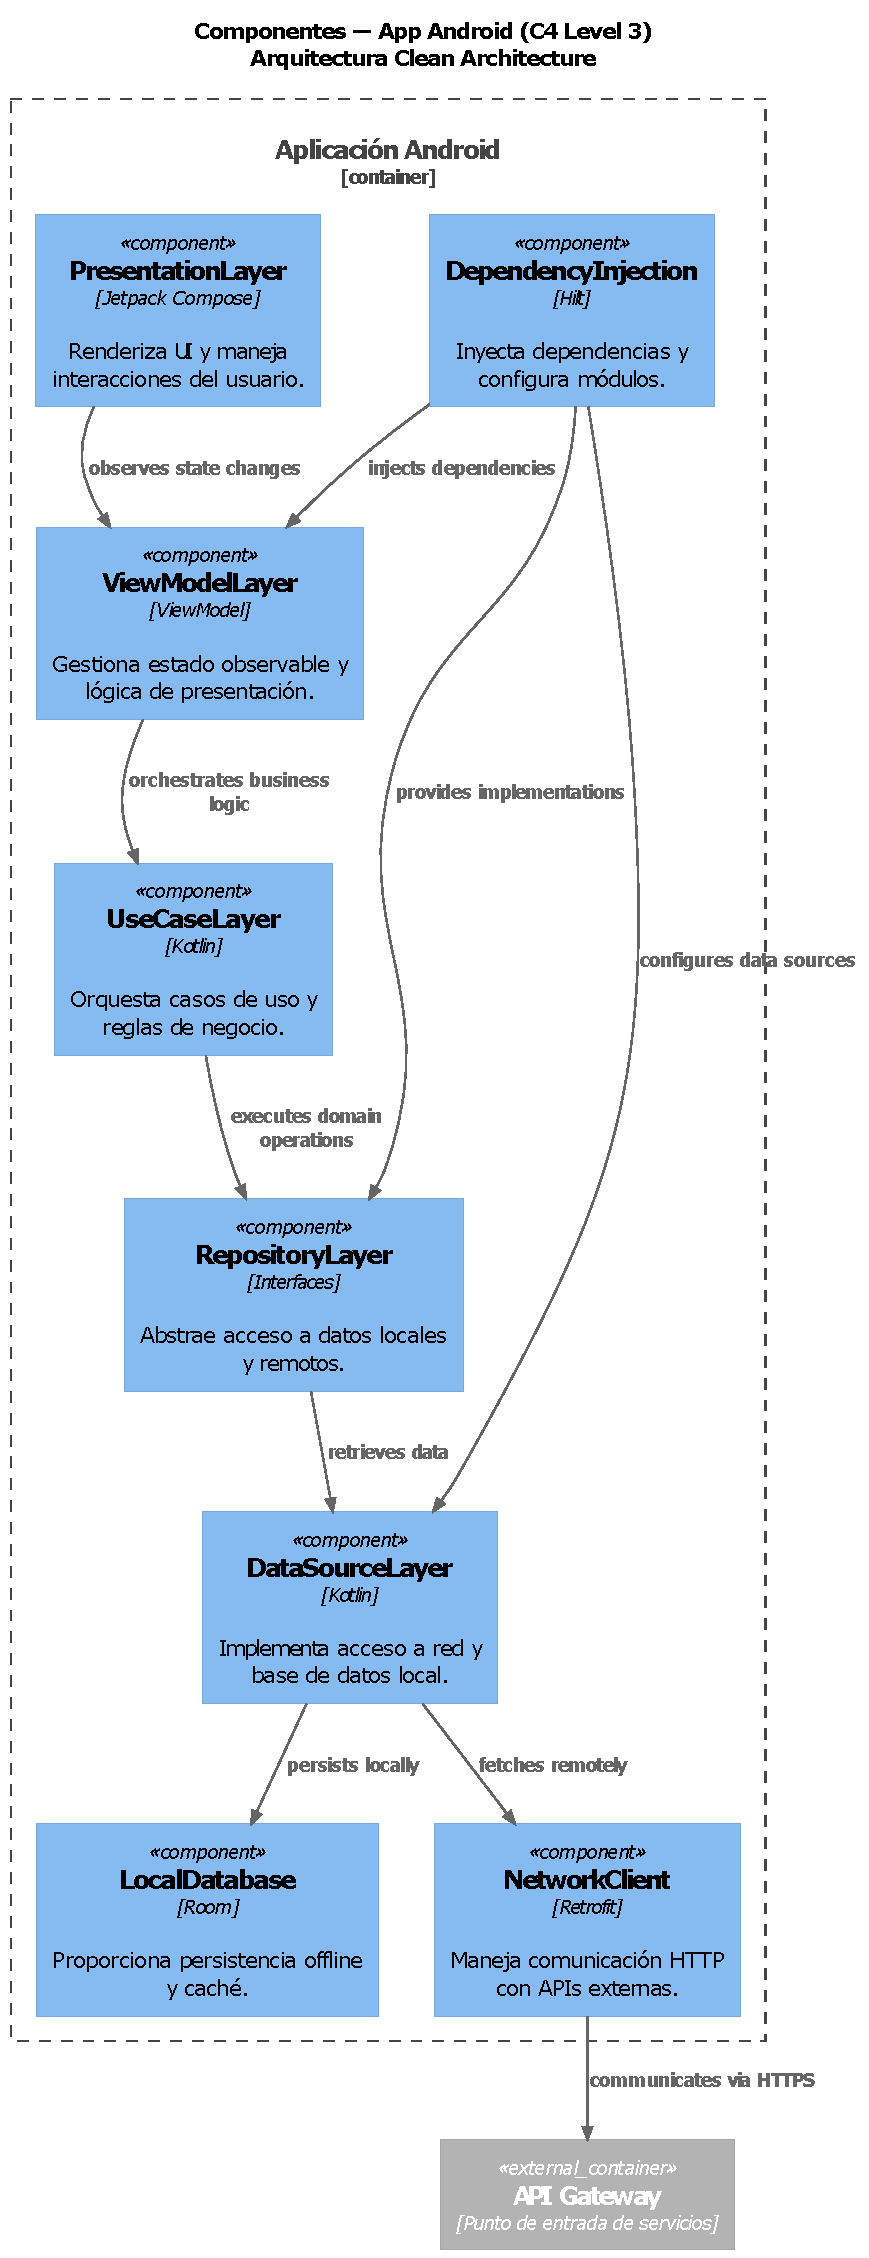
\includegraphics[width=0.85\textwidth,height=0.7\textheight,keepaspectratio]{figures/c4-model.level-3-components.android-app.pdf}
    \caption{Diagrama de componentes del cliente móvil (Android/Kotlin)}
    \label{fig:components_android}
\end{figure}

\begin{figure}[H]
    \centering
    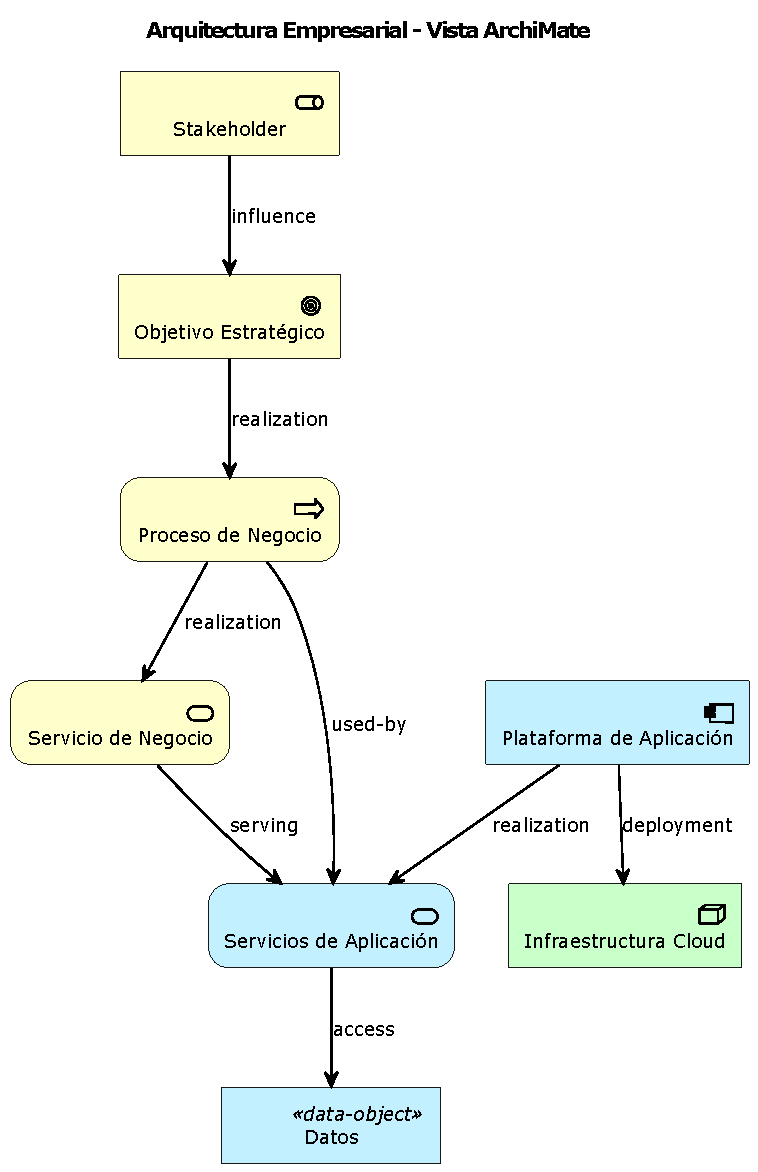
\includegraphics[width=0.85\textwidth,height=0.7\textheight,keepaspectratio]{figures/enterprise.archimate.pdf}
    \caption{Diagrama de arquitectura empresarial (ArchiMate)}
    \label{fig:enterprise_archimate}
\end{figure}

\begin{figure}[H]
    \centering
    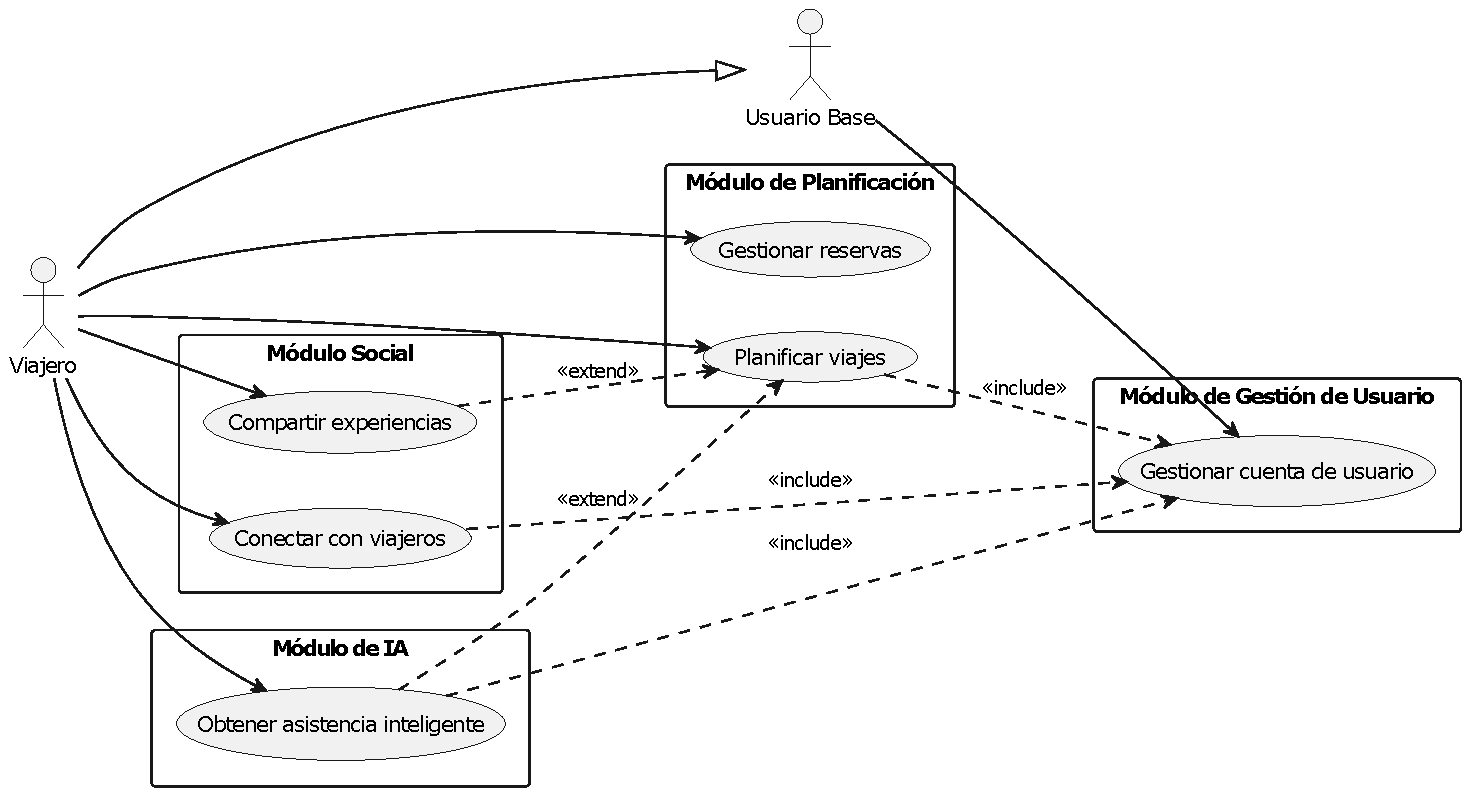
\includegraphics[width=0.85\textwidth,height=0.6\textheight,keepaspectratio]{figures/uml.behavior.use-cases.pdf}
    \caption{Diagrama de casos de uso del sistema}
    \label{fig:use_cases}
\end{figure}

\begin{figure}[H]
    \centering
    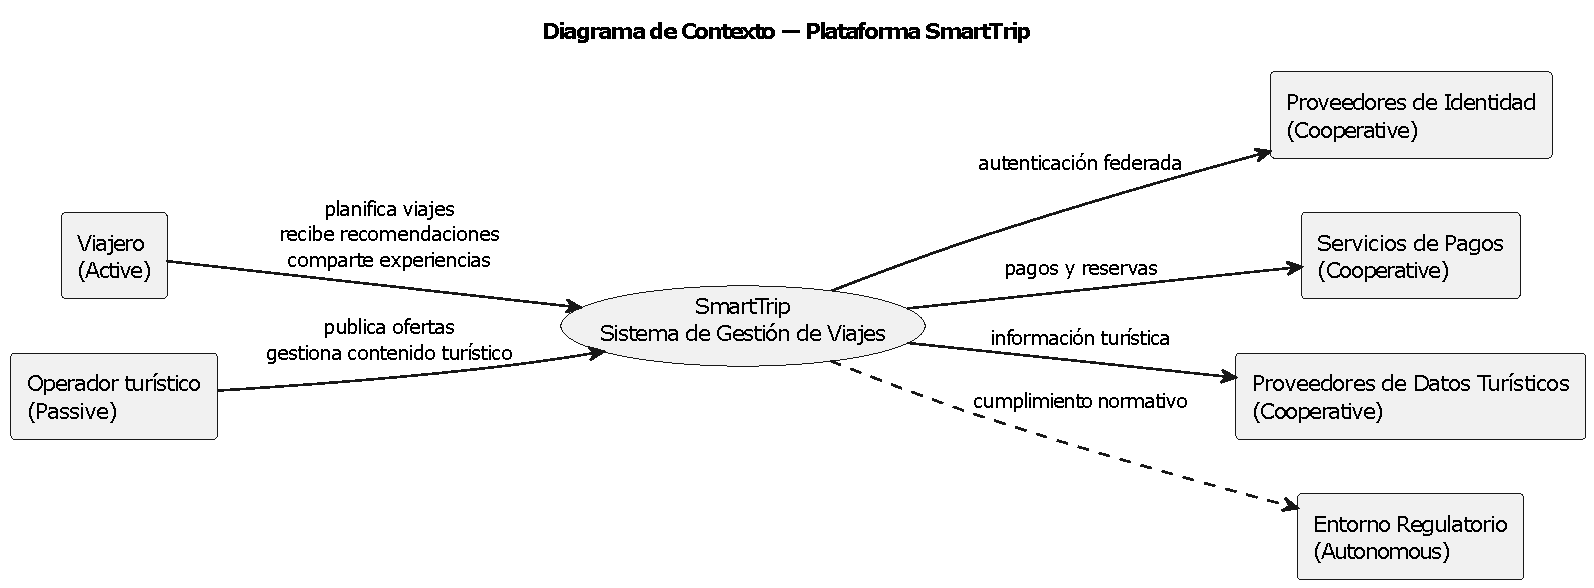
\includegraphics[width=0.85\textwidth,height=0.6\textheight,keepaspectratio]{figures/uml.context.system-context.pdf}
    \caption{Diagrama de contexto del sistema}
    \label{fig:system_context}
\end{figure}

\begin{figure}[H]
    \centering
    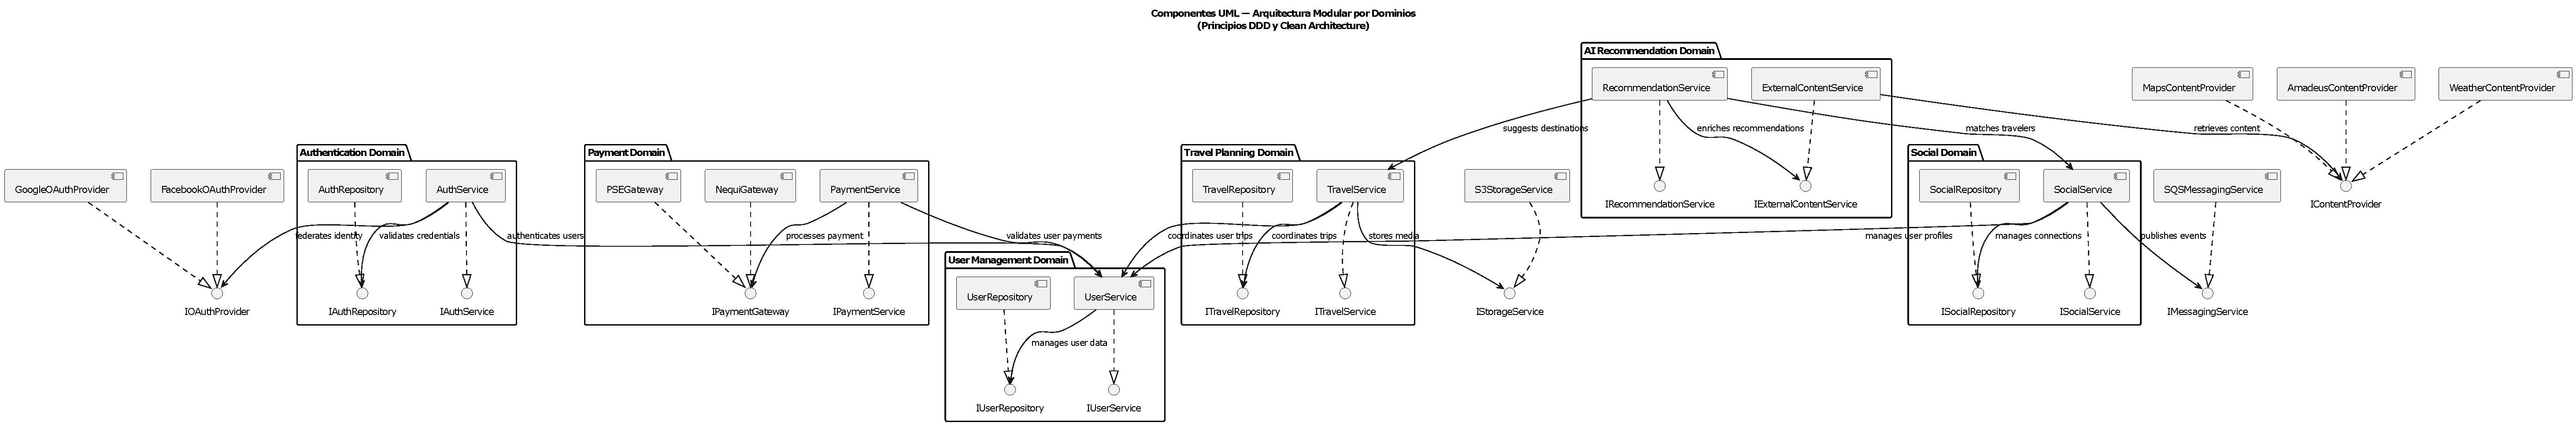
\includegraphics[width=0.85\textwidth,height=0.7\textheight,keepaspectratio]{figures/uml.structure.component-overview.pdf}
    \caption{Vista general de componentes del sistema}
    \label{fig:component_overview}
\end{figure}

\begin{figure}[H]
    \centering
    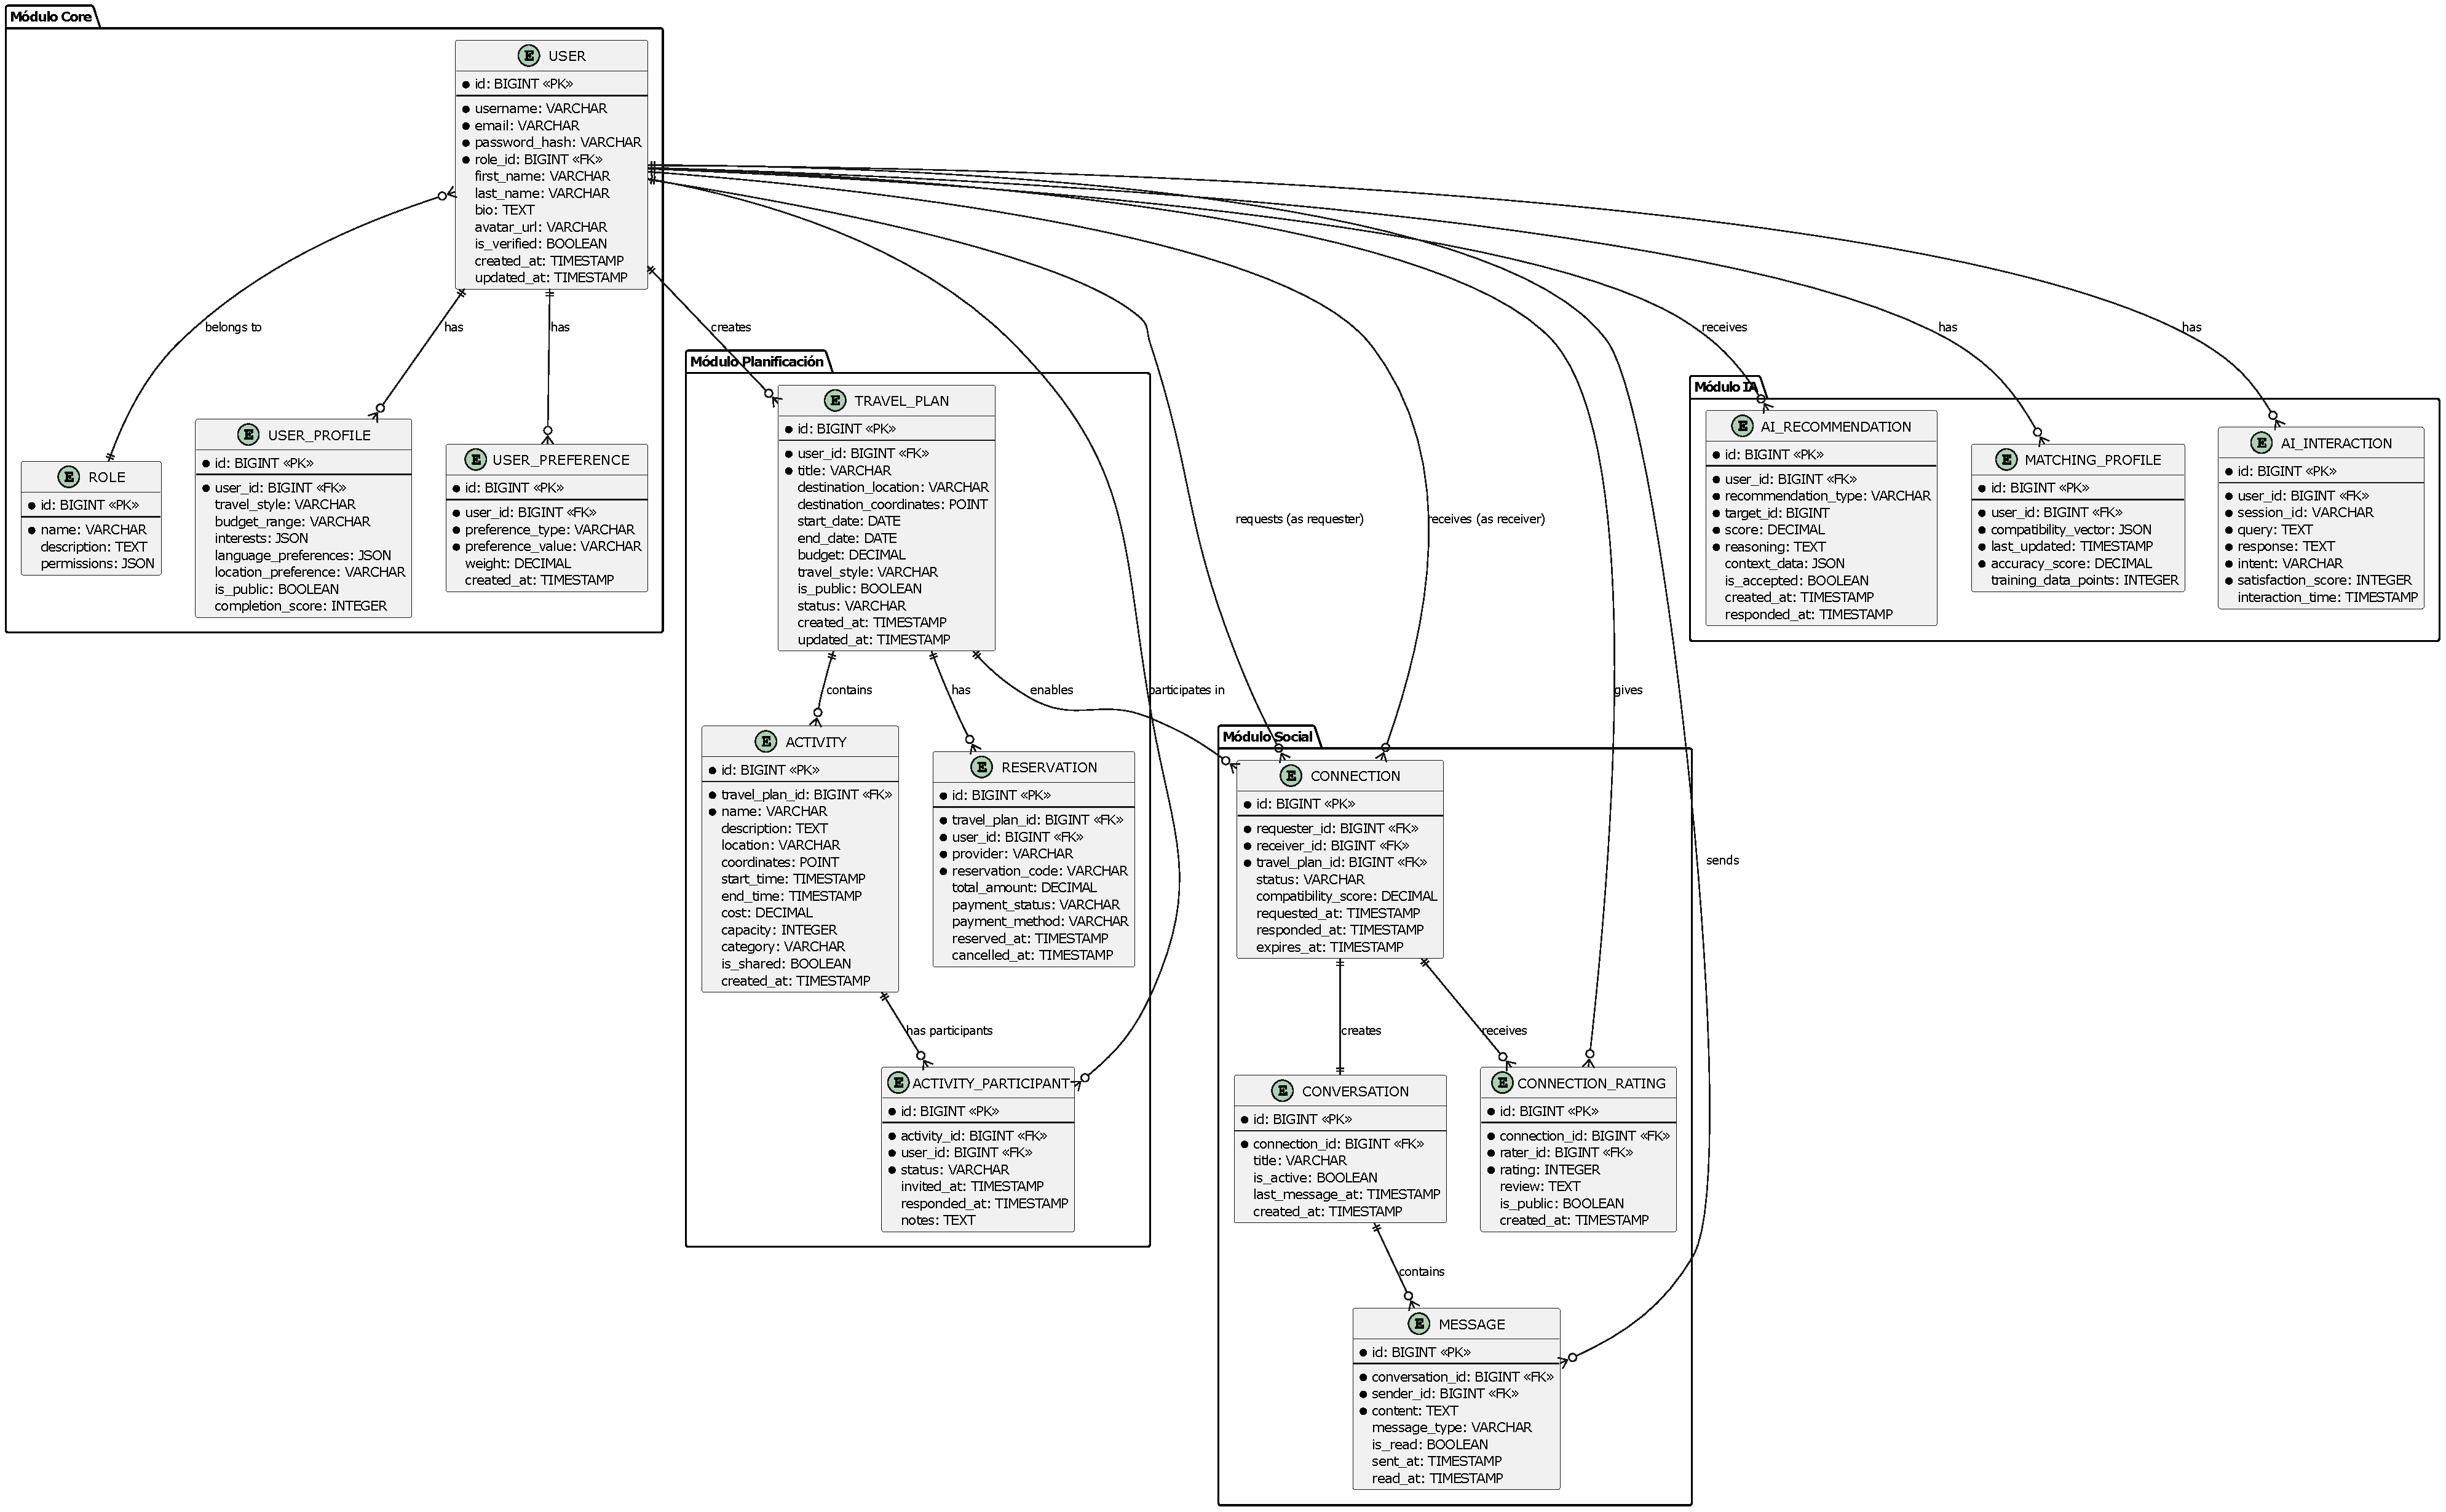
\includegraphics[width=0.85\textwidth,height=0.7\textheight,keepaspectratio]{figures/uml.structure.er-diagram.pdf}
    \caption{Diagrama entidad-relación del modelo de datos}
    \label{fig:er_diagram}
\end{figure}

\begin{figure}[H]
    \centering
    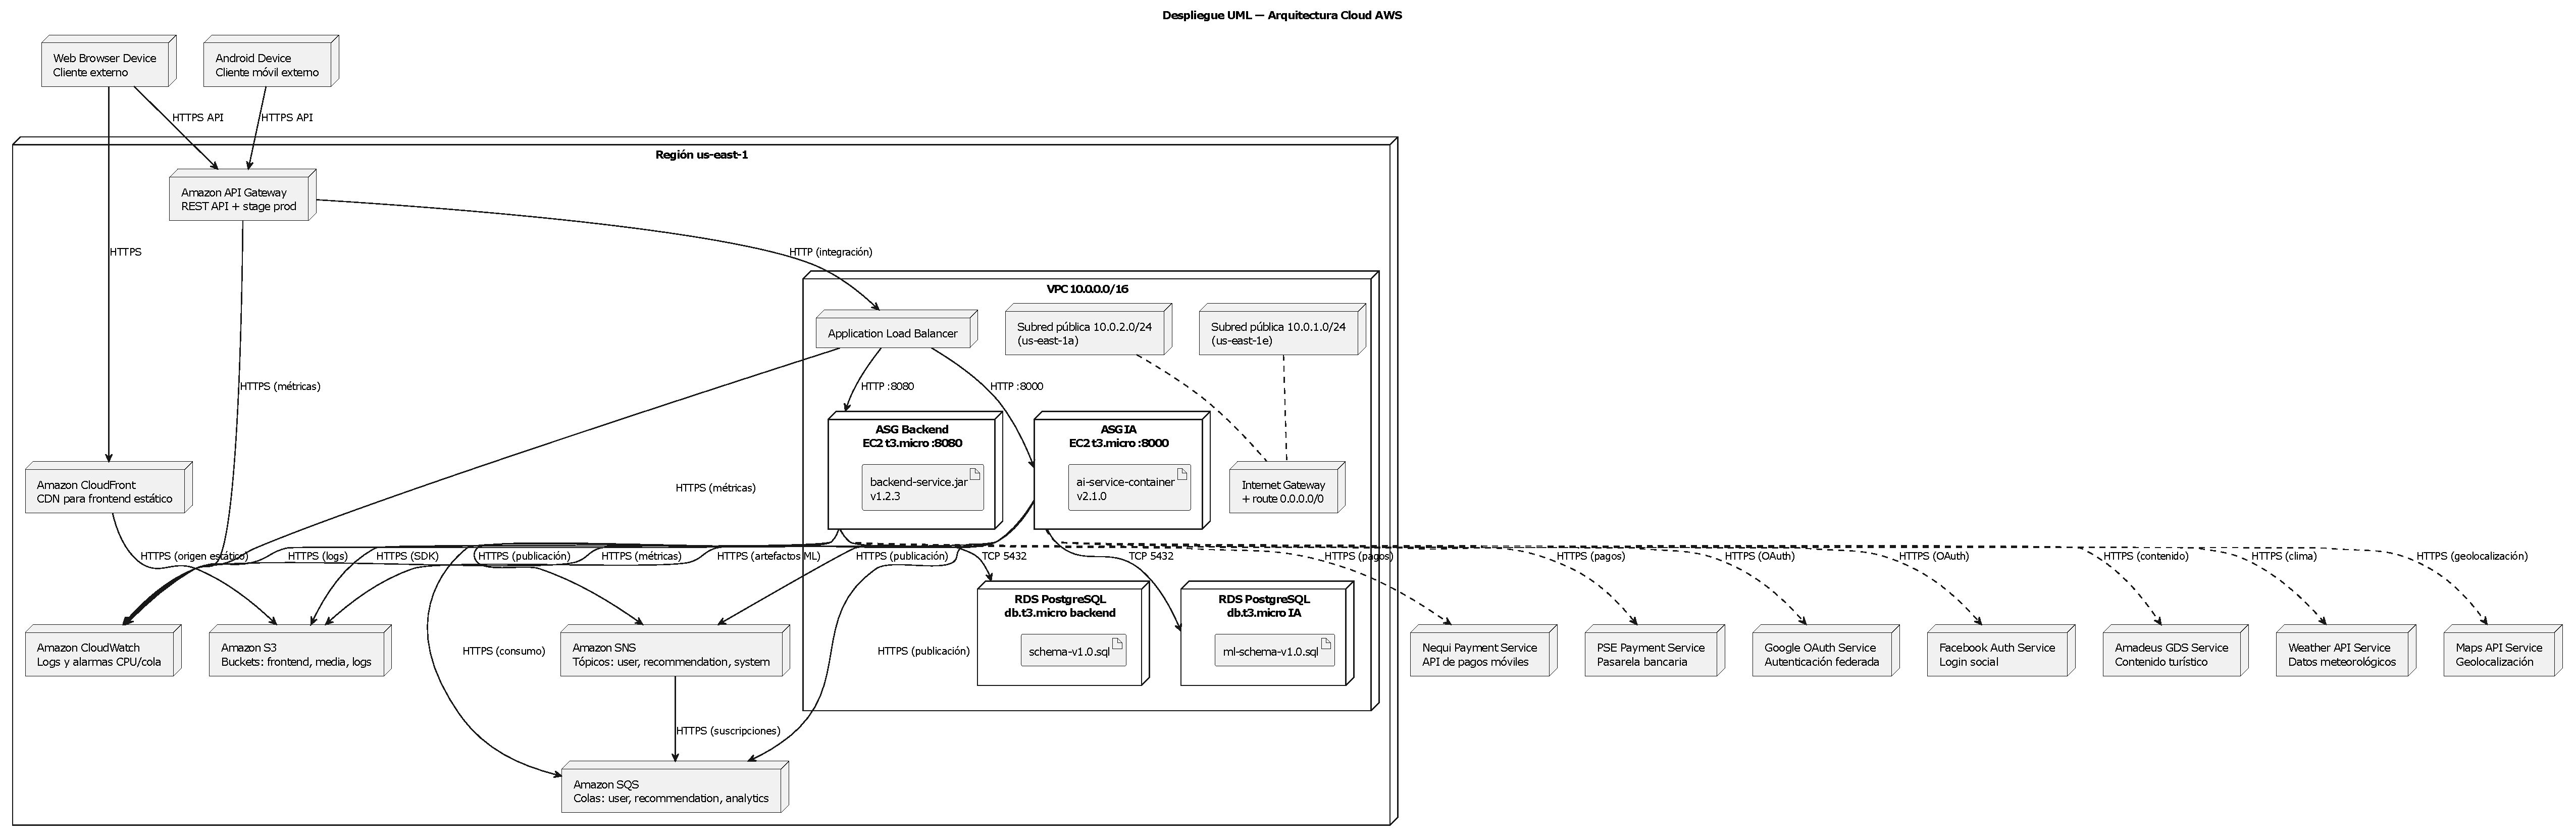
\includegraphics[width=0.85\textwidth,height=0.7\textheight,keepaspectratio]{figures/uml.deployment..deployment-diagram.pdf}
    \caption{Diagrama de despliegue del sistema}
    \label{fig:deployment_diagram}
\end{figure}

\begin{figure}[H]
    \centering
    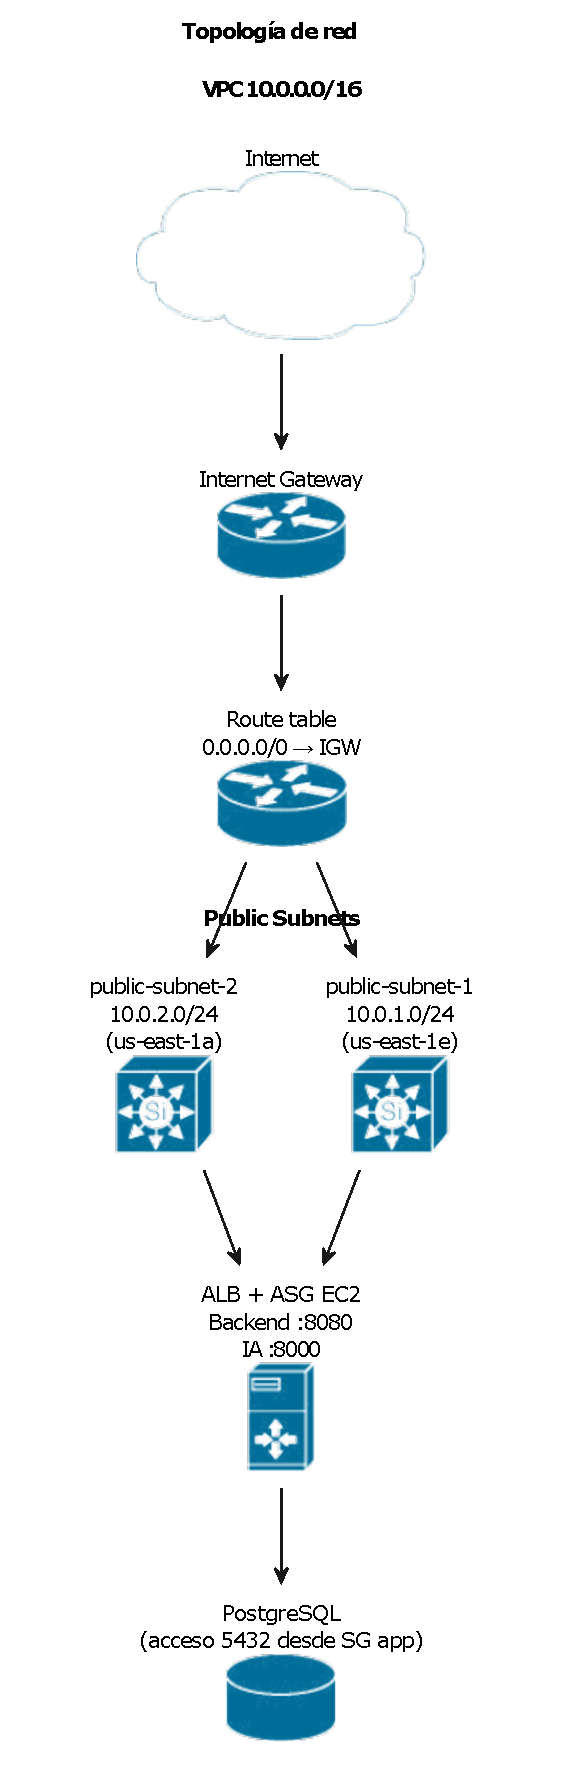
\includegraphics[width=0.85\textwidth,height=0.7\textheight,keepaspectratio]{figures/uml.deployment.network-topology.pdf}
    \caption{Topología de red en AWS}
    \label{fig:network_topology}
\end{figure}

\begin{figure}[H]
    \centering
    
\includegraphics[width=0.85\textwidth,height=0.6\textheight,keepaspectratio]{figures/uml.deployment.cicd-pipeline.pdf}
    \caption{Pipeline de CI/CD del sistema}
    \label{fig:cicd_pipeline}
\end{figure}

%================================================================================
\section{Análisis Sistémico del Proceso de Transformación Digital}
%================================================================================

El presente análisis sistémico revela las dinámicas complejas subyacentes en el proceso de transformación digital del sector turístico, identificando bucles de retroalimentación, arquetipos sistémicos y puntos de apalancamiento que determinan el éxito o fracaso de la implementación.

\subsection{Bucles Causales Fundamentales}

El sistema turístico digital presenta cinco bucles de retroalimentación principales que gobiernan su comportamiento:

\subsubsection{Bucle R1: Espiral de Soledad del Viajero}

\textbf{Tipo:} Refuerzo Negativo

\textbf{Variables:} Viajeros aislados → Baja satisfacción → Menor uso → Datos insuficientes → Peor personalización → Viajeros aislados

\begin{figure}[H]
    \centering
    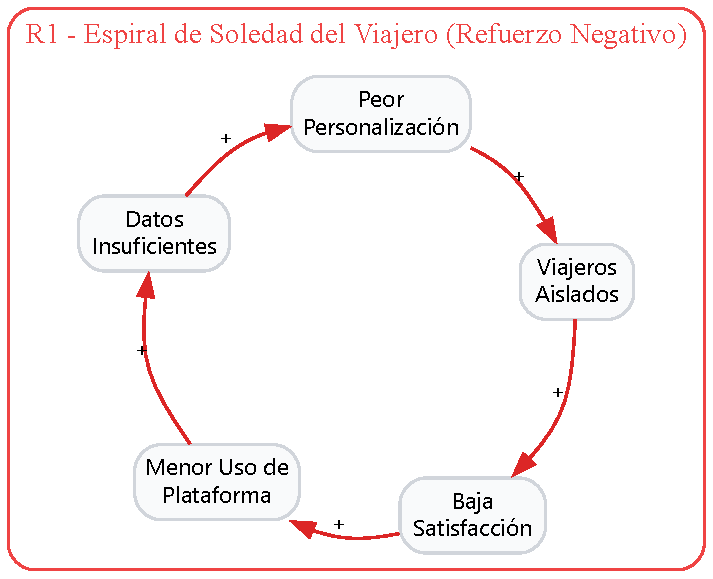
\includegraphics[width=0.85\textwidth,height=0.5\textheight,keepaspectratio]{figures/systems.atoms.loneliness-traveler.pdf}
    \caption{Bucle causal R1: Espiral de soledad del viajero}
    \label{fig:loneliness_loop}
\end{figure}

Este bucle representa una espiral descendente donde la falta de conexiones sociales reduce la satisfacción del usuario, disminuyendo el uso de la plataforma y limitando la disponibilidad de datos para mejorar los algoritmos de personalización.

\subsubsection{Bucle R2: Fragmentación de Experiencia}

\textbf{Tipo:} Refuerzo Negativo

\textbf{Variables:} Experiencias fragmentadas → Pérdida de contexto → Ineficiencia en planificación → Menor engagement → Reducida colaboración → Más fragmentación

\begin{figure}[H]
    \centering
    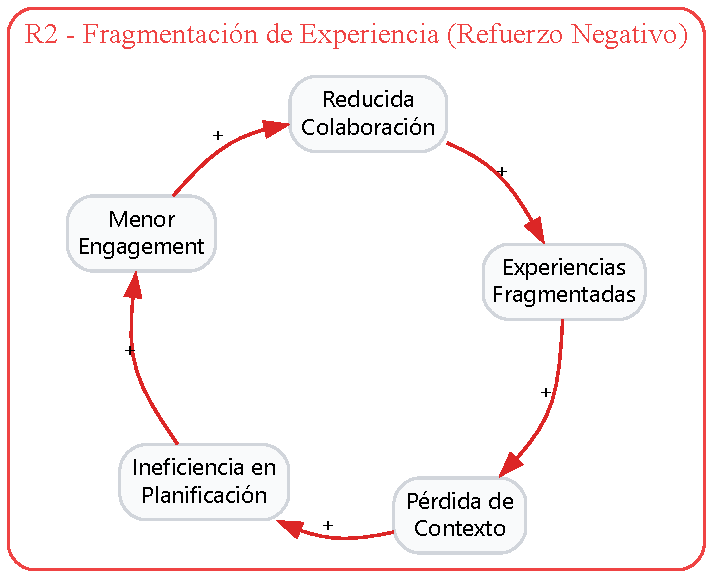
\includegraphics[width=0.85\textwidth,height=0.5\textheight,keepaspectratio]{figures/systems.atoms.experience-fragmentation.pdf}
    \caption{Bucle causal R2: Fragmentación de experiencia}
    \label{fig:fragmentation_loop}
\end{figure}

La separación entre las fases de planificación, ejecución y socialización del viaje genera una pérdida de contexto continuo, reduciendo la efectividad de las conexiones sociales y la colaboración entre viajeros.

\subsubsection{Bucle R3: Limitación de Datos de Matching}

\textbf{Tipo:} Refuerzo Negativo

\textbf{Variables:} Datos limitados → Algoritmos pobres → Baja precisión → Menor confianza → Menor participación → Menos datos

\begin{figure}[H]
    \centering
    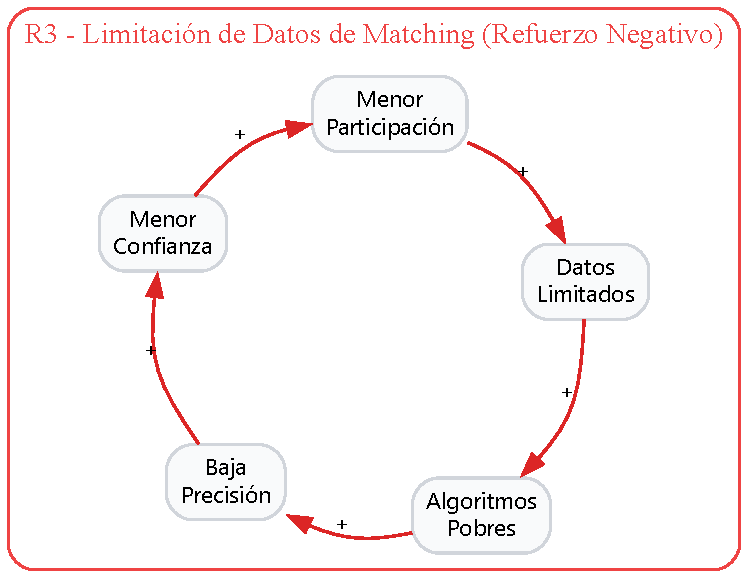
\includegraphics[width=0.85\textwidth,height=0.5\textheight,keepaspectratio]{figures/systems.atoms.data-matching-limits.pdf}
    \caption{Bucle causal R3: Limitación de datos de matching}
    \label{fig:data_matching_loop}
\end{figure}

La escasez de datos sociales limita la efectividad de los algoritmos de matching, creando un ciclo de desconfianza que reduce la participación de los usuarios y perpetúa la limitación de datos.

\subsubsection{Bucle B1: Escalabilidad de Personalización}

\textbf{Tipo:} Balanceo

\textbf{Variables:} Complejidad de matching → Recursos computacionales → Tiempo de respuesta → Experiencia usuario → Adopción → Limitación escala

\begin{figure}[H]
    \centering
    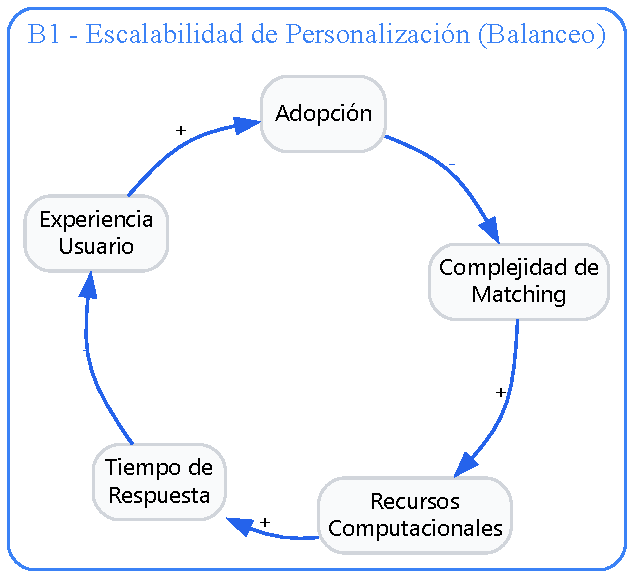
\includegraphics[width=0.85\textwidth,height=0.5\textheight,keepaspectratio]{figures/systems.atoms.personalization-scaling.pdf}
    \caption{Bucle causal B1: Escalabilidad de personalización}
    \label{fig:scalability_loop}
\end{figure}

La complejidad computacional del matching multidimensional crea restricciones de rendimiento que afectan la experiencia del usuario y limitan la adopción masiva de la plataforma.

\subsubsection{Bucle R4: Validación Social Post-Viaje}

\textbf{Tipo:} Refuerzo Positivo

\textbf{Variables:} Experiencias compartidas → Datos de validación → Mejora de algoritmos → Mejor matching → Más experiencias exitosas

\begin{figure}[H]
    \centering
    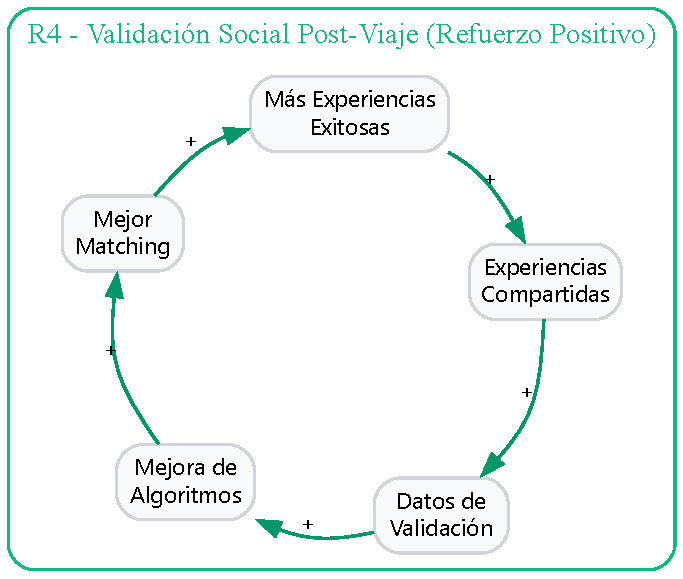
\includegraphics[width=0.85\textwidth,height=0.5\textheight,keepaspectratio]{figures/systems.atoms.post-trip-social-validation.pdf}
    \caption{Bucle causal R4: Validación social post-viaje}
    \label{fig:validation_loop}
\end{figure}

Este bucle positivo representa el potencial de crecimiento del sistema mediante el aprendizaje continuo de experiencias compartidas, mejorando progresivamente la calidad del matching y generando más experiencias exitosas.

\subsection{Arquetipos Sistémicos Identificados}

El análisis revela cuatro arquetipos sistémicos principales que gobiernan el comportamiento del sistema turístico digital:

\subsubsection{Límites del Crecimiento}

El sistema exhibe un claro arquetipo de ``Límites del Crecimiento'' donde el bucle de refuerzo positivo R4 impulsa el crecimiento inicial a través de experiencias exitosas, pero se encuentra con múltiples límites que frenan este crecimiento:

\begin{itemize}
\item \textbf{Límite principal (R1):} La espiral de soledad del viajero crea un ciclo vicioso que reduce la satisfacción y el uso de la plataforma
\item \textbf{Límite de datos (R3):} La limitación de datos de matching crea una barrera fundamental para la personalización efectiva
\item \textbf{Límite técnico (B1):} La escalabilidad de personalización introduce restricciones computacionales que afectan la experiencia del usuario
\end{itemize}

\subsubsection{Desplazamiento de la Carga}

Se observa un patrón de ``Desplazamiento de la Carga'' donde la solución sintomática (R4 - Validación Social Post-Viaje) alivia temporalmente los síntomas pero debilita la capacidad del sistema para resolver el problema fundamental:

\begin{itemize}
\item \textbf{Solución sintomática:} R4 proporciona validación social y mejora temporal de matching
\item \textbf{Problema fundamental:} R1 (Soledad del Viajero) y R2 (Fragmentación de Experiencia) representan las causas raíz
\item \textbf{Efecto secundario:} La dependencia en R4 reduce la motivación para abordar los problemas estructurales
\end{itemize}

\subsubsection{Erosión de Metas}

El sistema muestra erosión gradual de las metas originales a través de la degradación progresiva de estándares:

\begin{itemize}
\item \textbf{Meta original:} Proporcionar experiencias de viaje personalizadas y conectadas
\item \textbf{Erosión:} R1 y R3 degradan progresivamente la calidad de la experiencia y personalización
\item \textbf{Aceptación del deterioro:} B1 muestra cómo el sistema se adapta a limitaciones técnicas aceptando estándares menores
\end{itemize}

\subsubsection{Éxito a los Exitosos}

Se crea una brecha creciente entre usuarios exitosos y usuarios en dificultades:

\begin{itemize}
\item \textbf{Ganadores:} Usuarios que participan en R4 obtienen mejores experiencias y más matching
\item \textbf{Perdedores:} Usuarios atrapados en R1 y R2 reciben servicios degradados
\item \textbf{Reforzamiento:} R4 mejora los algoritmos para los ya exitosos, mientras que R1 y R3 empeoran para los marginados
\end{itemize}

\subsection{Puntos de Apalancamiento del Sistema}

El análisis sistémico identifica tres puntos de apalancamiento de alto impacto para intervenir efectivamente en el sistema:

\subsubsection{Intervención en Datos de Matching (R3)}

\textbf{Impacto:} Afecta directamente R1, R4 y B1

\textbf{Estrategia:} Implementar estrategias de adquisición de datos y participación

\textbf{Resultado esperado:} Mejora general del sistema y rompe múltiples ciclos negativos

\subsubsection{Integración de Experiencias (R2)}

\textbf{Impacto:} Reduce fragmentación y facilita conexiones sociales

\textbf{Estrategia:} Diseñar flujos integrados que promuevan colaboración natural

\textbf{Resultado esperado:} Ataca directamente la soledad y mejora engagement

\subsubsection{Optimización de Algoritmos (R4 × B1)}

\textbf{Impacto:} Balancea crecimiento con sostenibilidad técnica

\textbf{Estrategia:} Desarrollar algoritmos eficientes que escalen bien

\textbf{Resultado esperado:} Sostenibilidad del crecimiento a largo plazo

\begin{figure}[H]
    \centering
    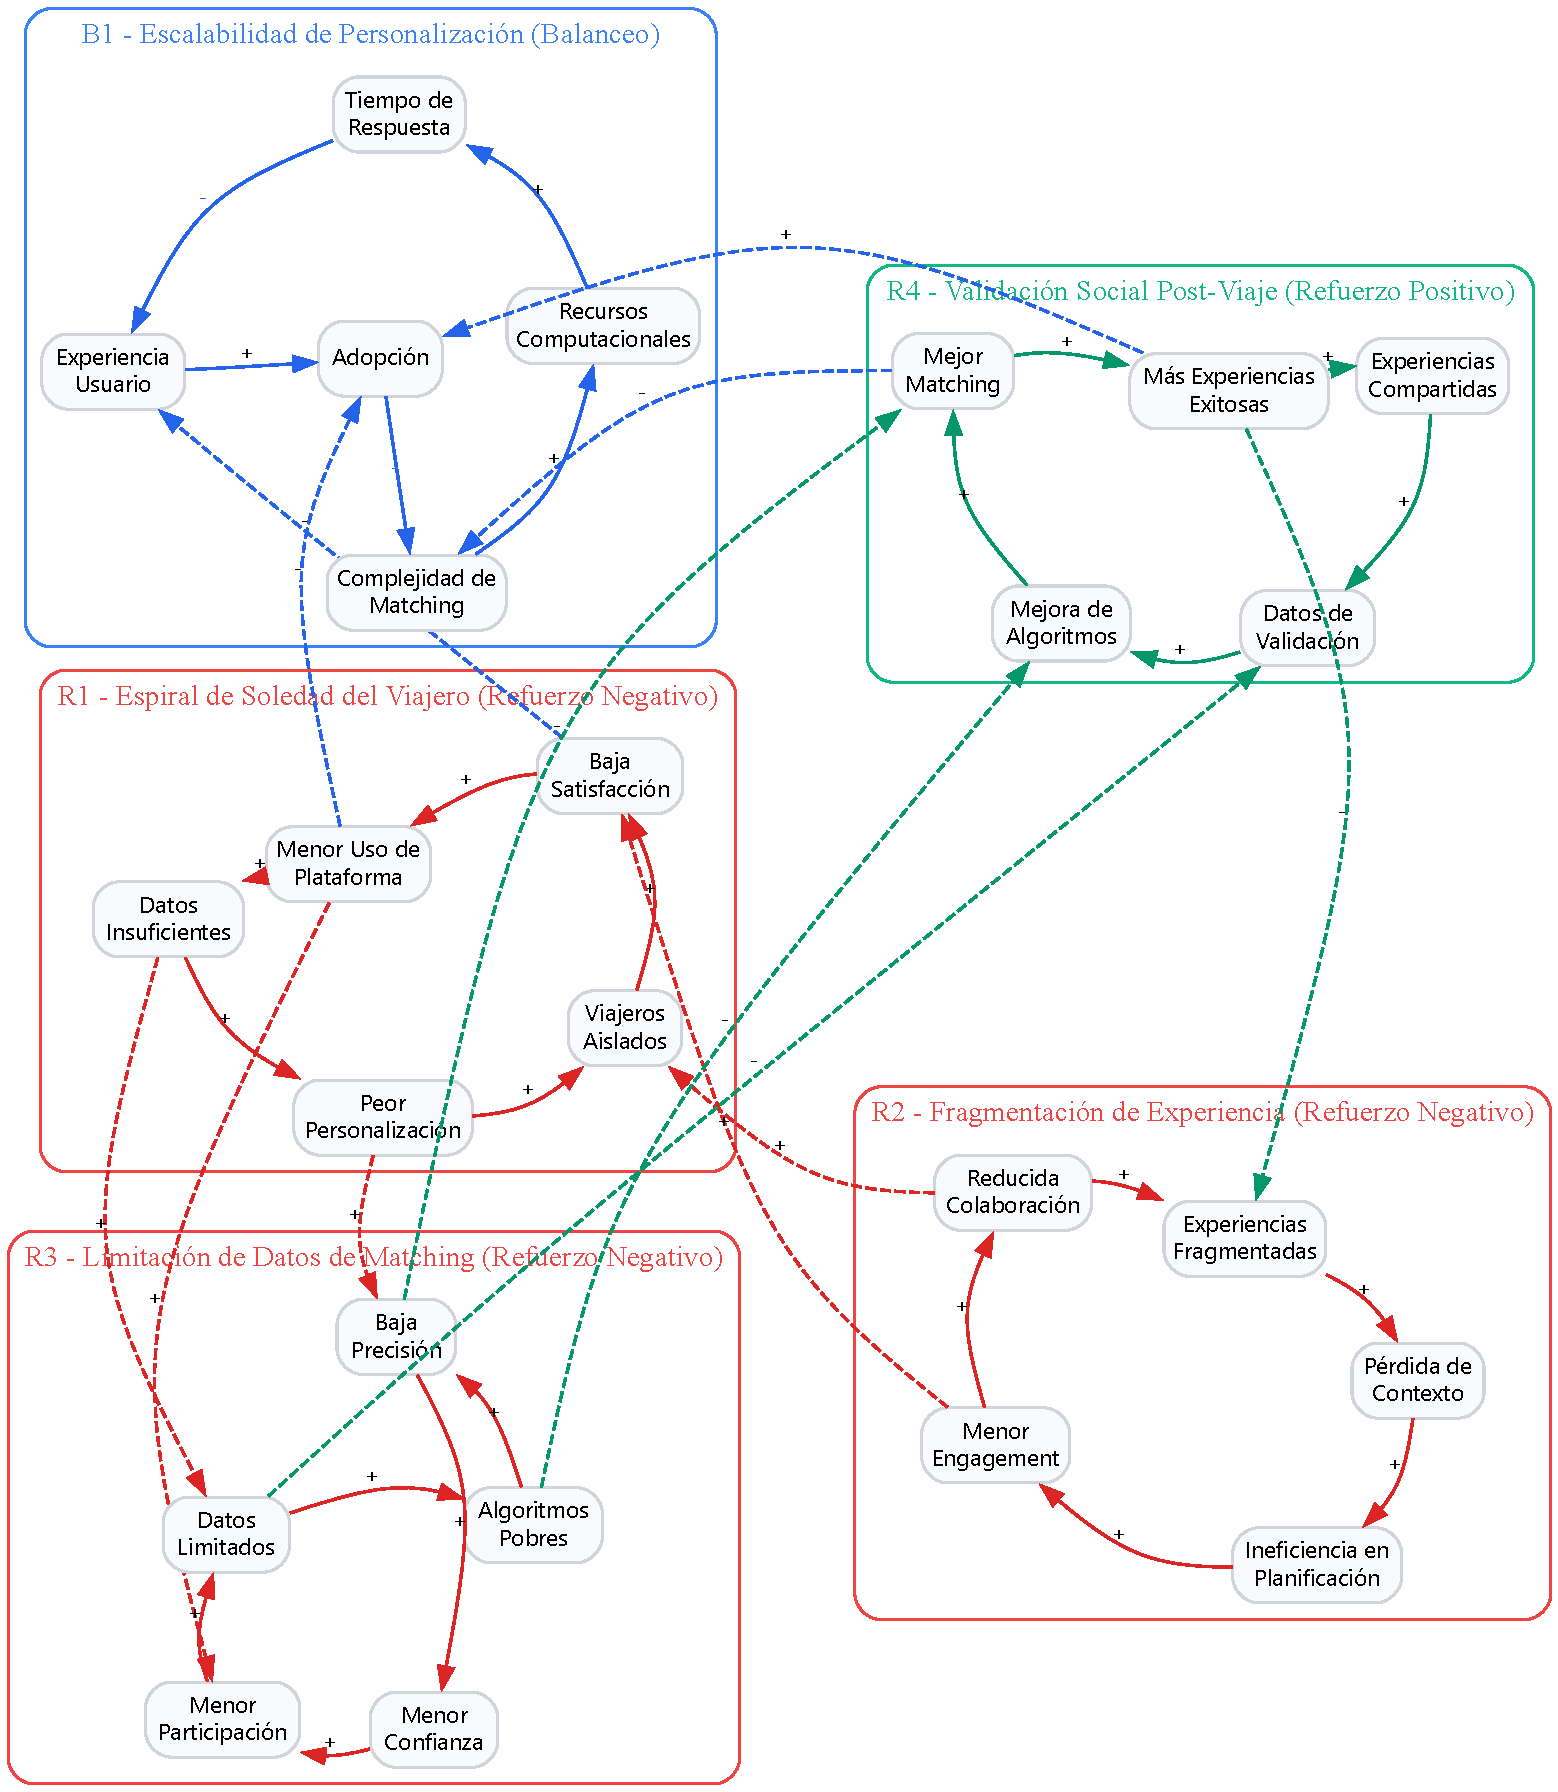
\includegraphics[width=0.85\textwidth,height=0.7\textheight,keepaspectratio]{figures/systems.maps.systemic-model.pdf}
    \caption{Modelo sistémico integrado con interacciones entre bucles causales}
    \label{fig:systemic_model}
\end{figure}

\subsection{Implicaciones Estratégicas para la Transformación Digital}

El análisis sistémico proporciona insights estratégicos cruciales para la implementación exitosa de la transformación digital:

\subsubsection{Enfoque en Causa Raíz}

Abordar aislamiento (R1) y fragmentación (R2) en lugar de solo optimización algorítmica superficial. Las intervenciones deben centrarse en:

\begin{itemize}
\item Programas de onboarding que prevengan el aislamiento inicial
\item Flujos de trabajo integrados que mantengan contexto continuo
\item Mecanismos de conexión natural entre usuarios
\end{itemize}

\subsubsection{Estrategia de Datos}

Priorizar adquisición de datos y participación para romper restricciones R3:

\begin{itemize}
\item Incentivos para compartir experiencias y preferencias
\item Mecanismos de validación social que generen datos de calidad
\item Procesamiento de datos que mejore progresivamente los algoritmos
\end{itemize}

\subsubsection{Crecimiento Sostenible}

Balancear expansión R4 con limitaciones técnicas B1:

\begin{itemize}
\item Optimización algorítmica para reducir complejidad computacional
\item Arquitectura escalable que soporte crecimiento sostenible
\item Métricas de calidad que detecten erosión de metas
\end{itemize}

\subsection{Recomendaciones de Intervención}

\subsubsection{Prioridad Alta: Romper Ciclos de Refuerzo Negativo}

\begin{enumerate}
\item \textbf{Implementar programas de onboarding} que prevengan el aislamiento inicial (R1)
\item \textbf{Crear incentivos de participación} para aumentar datos disponibles (R3)
\item \textbf{Diseñar experiencias integradas} que faciliten colaboración natural (R2)
\end{enumerate}

\subsubsection{Prioridad Media: Optimizar Crecimiento Positivo}

\begin{enumerate}
\item \textbf{Mejorar eficiencia algorítmica} para sostener R4 sin sobrecargar B1
\item \textbf{Desarrollar mecanismos de redistribución} para evitar ``éxito a los exitosos''
\item \textbf{Establecer métricas de calidad} para detectar erosión de metas
\end{enumerate}

\subsubsection{Prioridad Baja: Monitoreo y Adaptación}

\begin{enumerate}
\item \textbf{Implementar dashboards sistémicos} para visualizar dinámicas
\item \textbf{Crear sistemas de alerta temprana} para ciclos problemáticos
\item \textbf{Establecer revisiones periódicas} de arquetipos emergentes
\end{enumerate}

%================================================================================
\section{Atributos de Calidad del Sistema}
%================================================================================

Los atributos de calidad del sistema se han diseñado como escenarios verificables que orientan las decisiones arquitectónicas y operativas. Los siguientes diagramas detallan cada atributo de calidad con sus respectivas estrategias de implementación:

\begin{figure}[H]
    \centering
    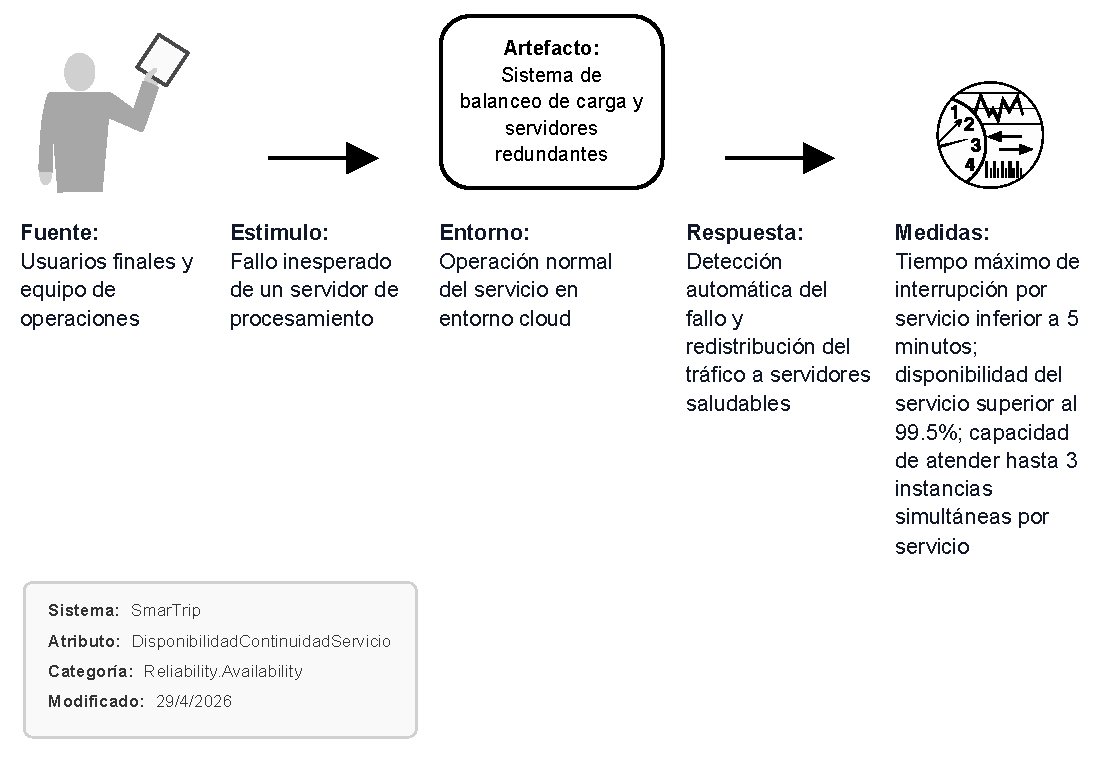
\includegraphics[width=0.85\textwidth,height=0.6\textheight,keepaspectratio]{figures/quality-attributes.SmarTrip_DisponibilidadContinuidadServicio.pdf}
    \caption{Disponibilidad y continuidad del servicio}
    \label{fig:availability}
\end{figure}

\begin{figure}[H]
    \centering
    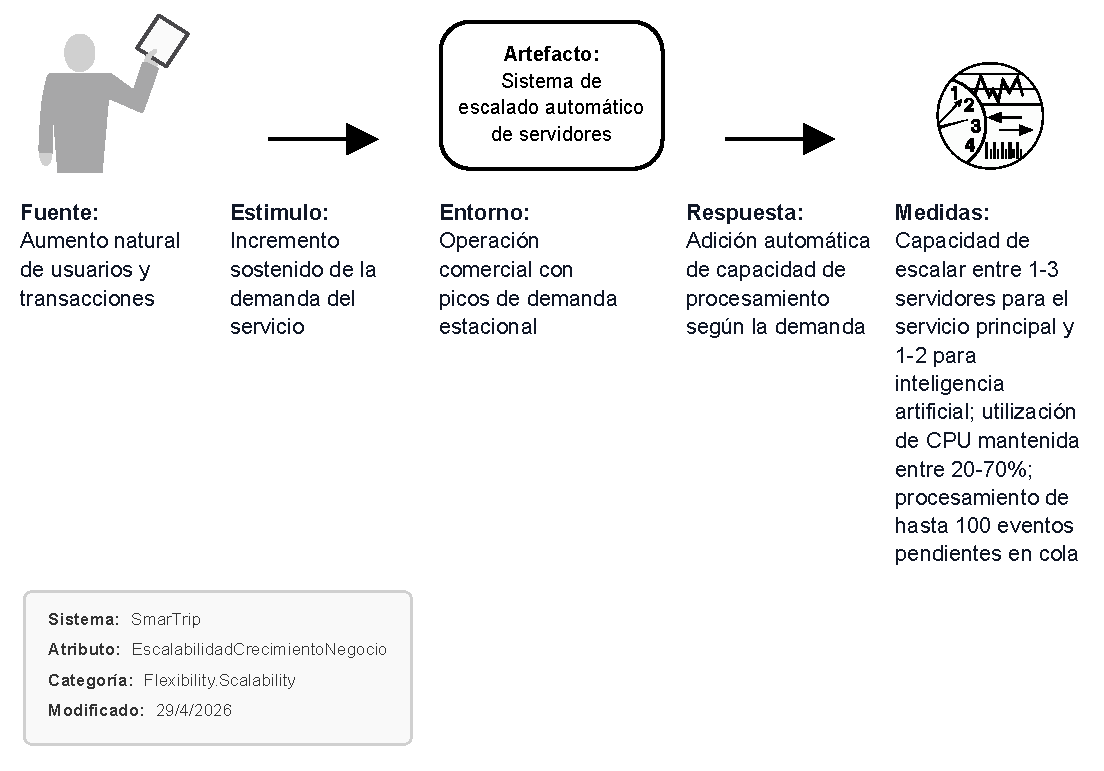
\includegraphics[width=0.85\textwidth,height=0.6\textheight,keepaspectratio]{figures/quality-attributes.SmarTrip_EscalabilidadCrecimientoNegocio.pdf}
    \caption{Escalabilidad y crecimiento del negocio}
    \label{fig:scalability}
\end{figure}

\begin{figure}[H]
    \centering
    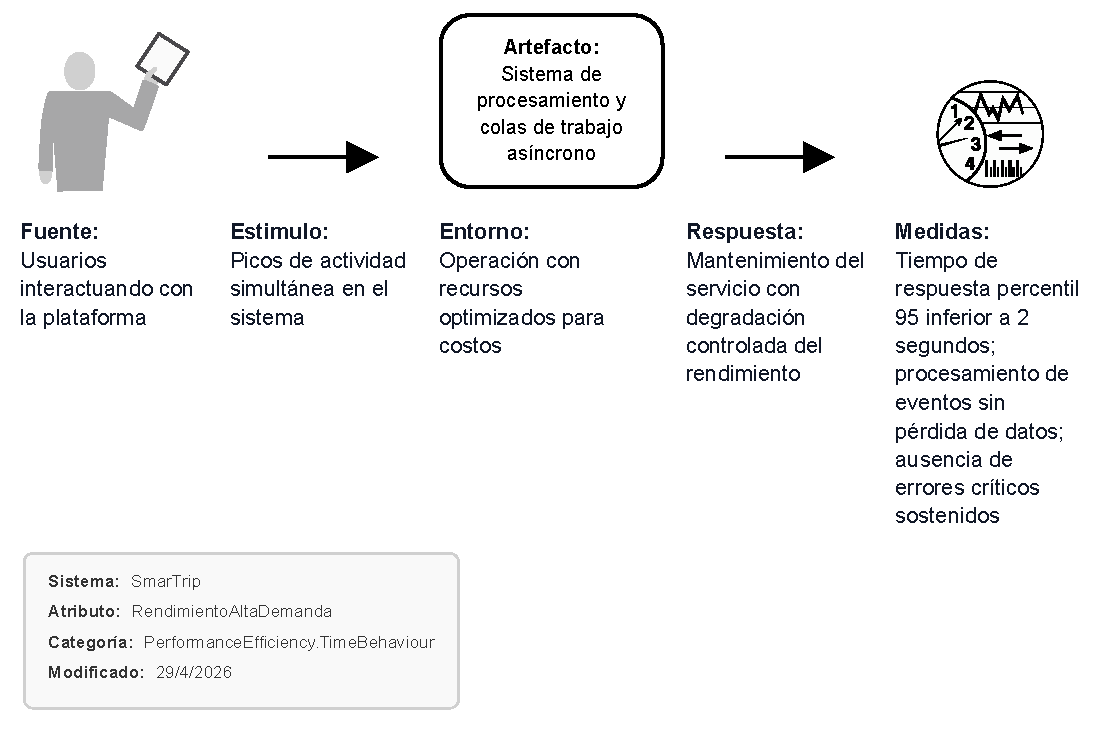
\includegraphics[width=0.85\textwidth,height=0.6\textheight,keepaspectratio]{figures/quality-attributes.SmarTrip_RendimientoAltaDemanda.pdf}
    \caption{Rendimiento bajo alta demanda}
    \label{fig:performance}
\end{figure}

\begin{figure}[H]
    \centering
    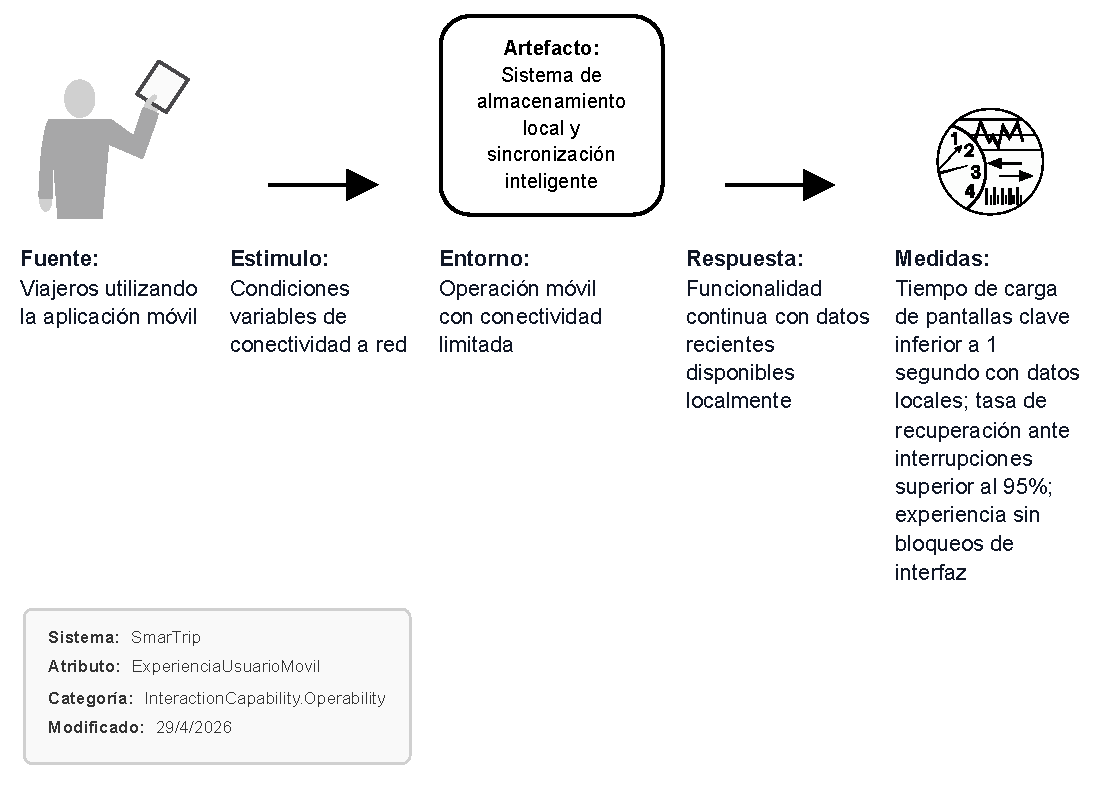
\includegraphics[width=0.85\textwidth,height=0.6\textheight,keepaspectratio]{figures/quality-attributes.SmarTrip_ExperienciaUsuarioMovil.pdf}
    \caption{Experiencia de usuario móvil}
    \label{fig:ux_mobile}
\end{figure}

\begin{figure}[H]
    \centering
    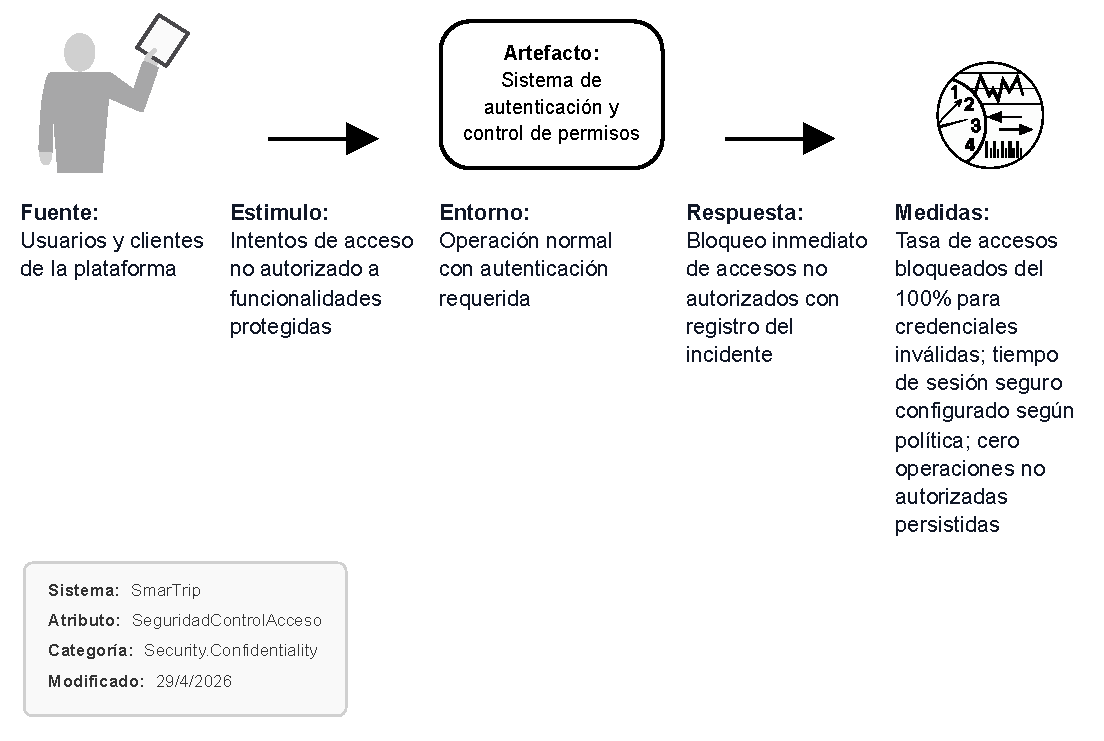
\includegraphics[width=0.85\textwidth,height=0.6\textheight,keepaspectratio]{figures/quality-attributes.SmarTrip_SeguridadControlAcceso.pdf}
    \caption{Seguridad y control de acceso}
    \label{fig:security_access}
\end{figure}

\begin{figure}[H]
    \centering
    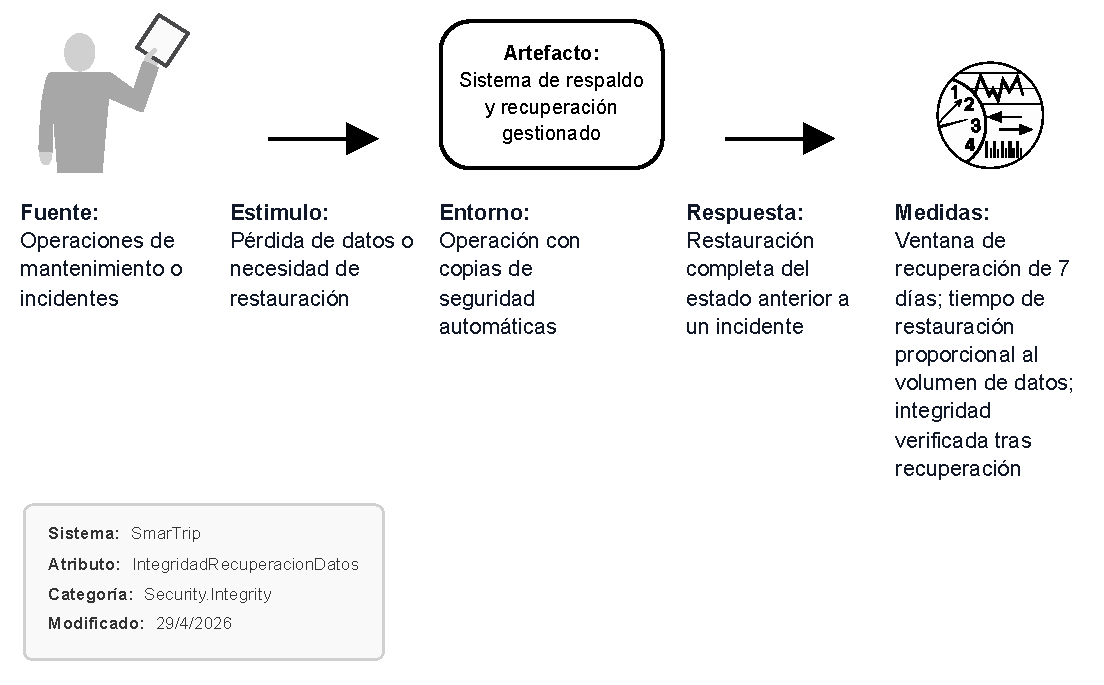
\includegraphics[width=0.85\textwidth,height=0.6\textheight,keepaspectratio]{figures/quality-attributes.SmarTrip_IntegridadRecuperacionDatos.pdf}
    \caption{Integridad y recuperación de datos}
    \label{fig:data_integrity}
\end{figure}

\begin{figure}[H]
    \centering
    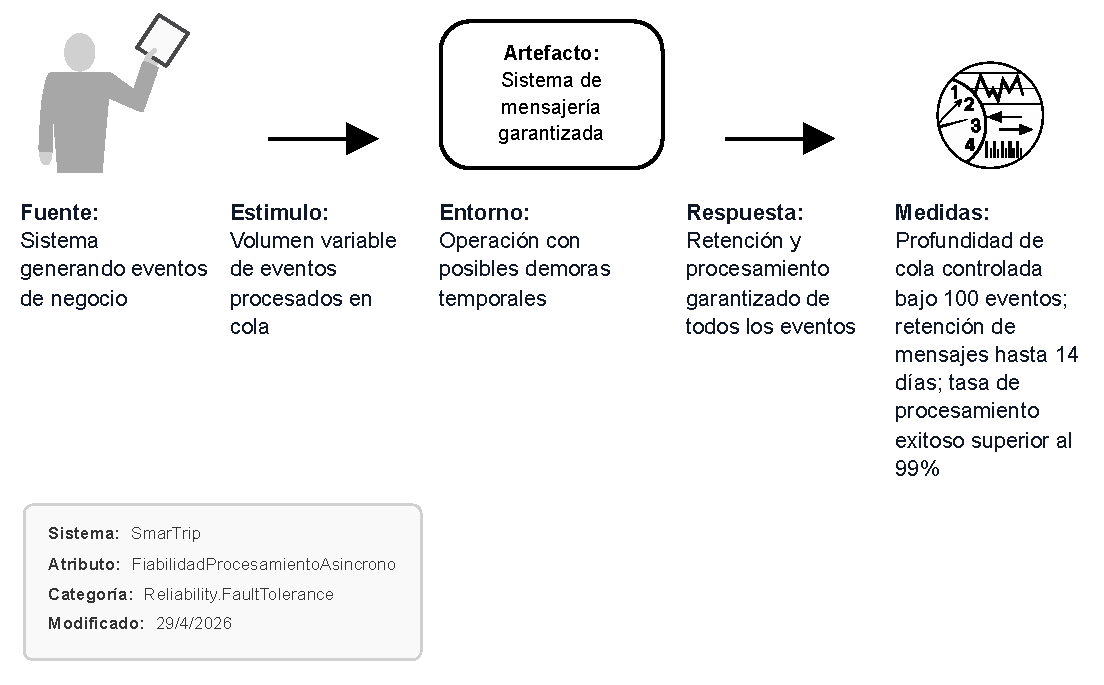
\includegraphics[width=0.85\textwidth,height=0.6\textheight,keepaspectratio]{figures/quality-attributes.SmarTrip_FiabilidadProcesamientoAsincrono.pdf}
    \caption{Fiabilidad del procesamiento asíncrono}
    \label{fig:async_reliability}
\end{figure}

\begin{figure}[H]
    \centering
    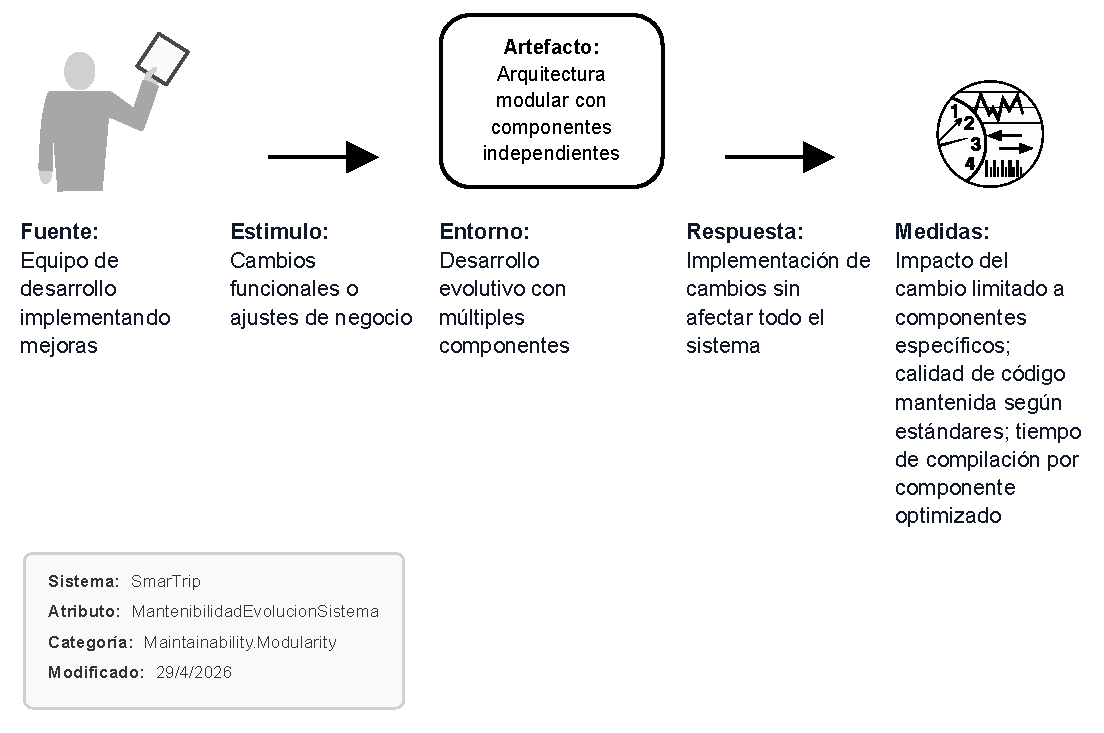
\includegraphics[width=0.85\textwidth,height=0.6\textheight,keepaspectratio]{figures/quality-attributes.SmarTrip_MantenibilidadEvolucionSistema.pdf}
    \caption{Mantenibilidad y evolución del sistema}
    \label{fig:maintainability}
\end{figure}

\begin{figure}[H]
    \centering
    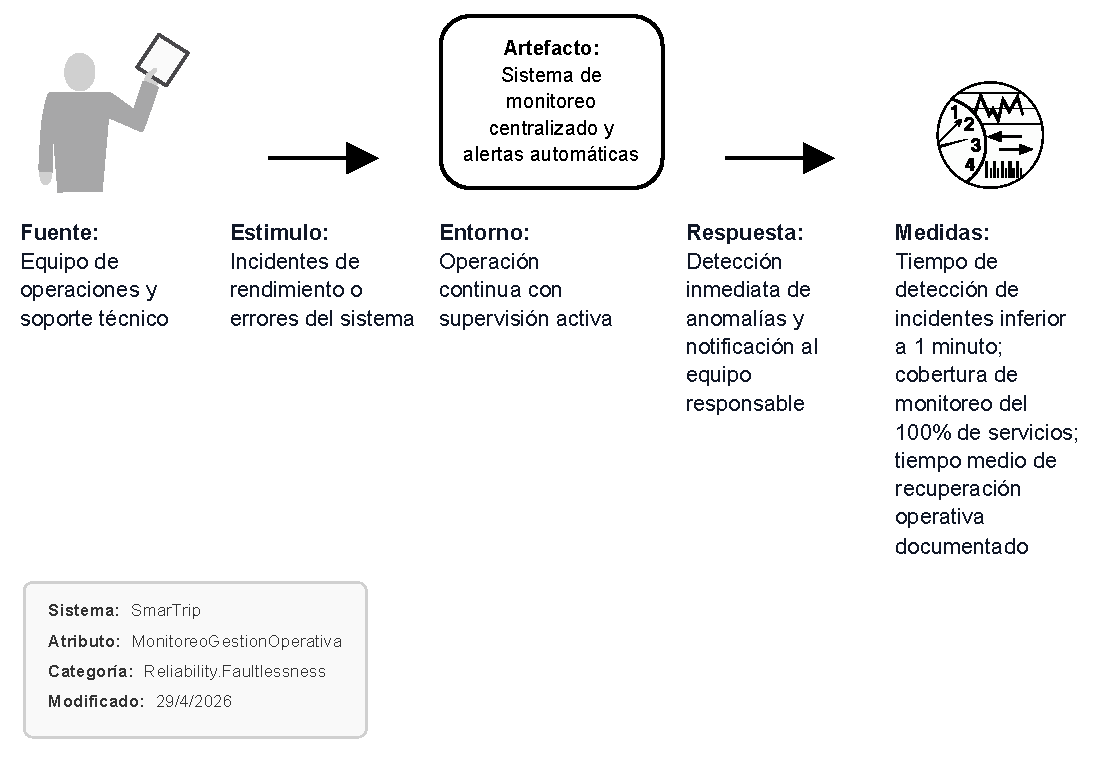
\includegraphics[width=0.85\textwidth,height=0.6\textheight,keepaspectratio]{figures/quality-attributes.SmarTrip_MonitoreoGestionOperativa.pdf}
    \caption{Monitoreo y gestión operativa}
    \label{fig:monitoring}
\end{figure}

\begin{figure}[H]
    \centering
    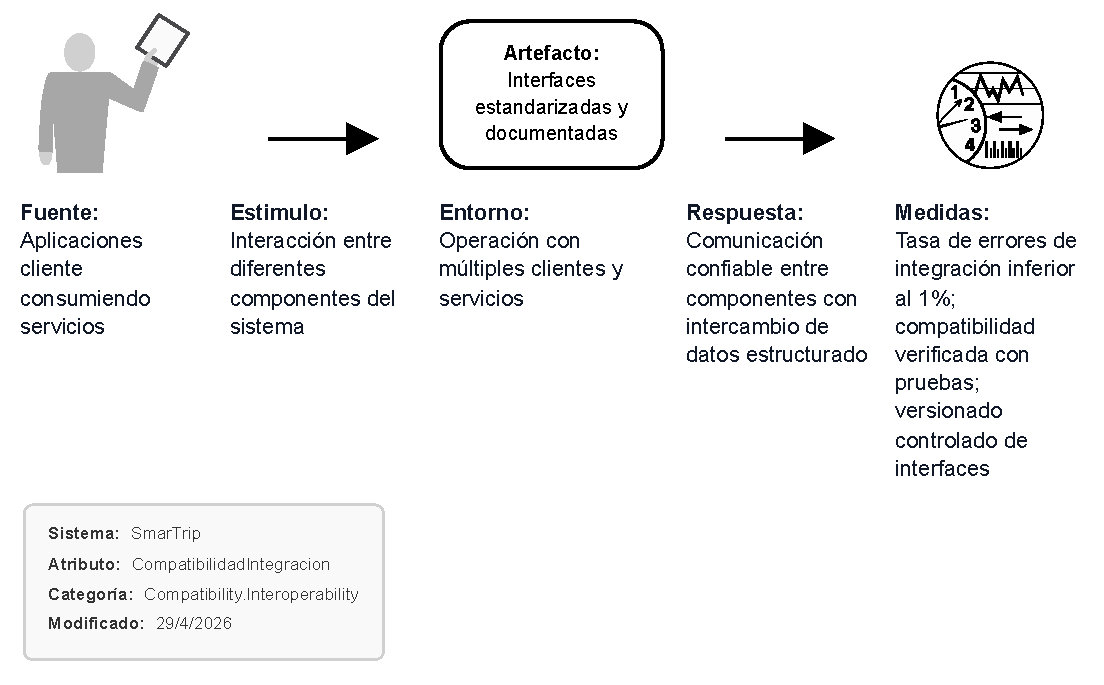
\includegraphics[width=0.85\textwidth,height=0.6\textheight,keepaspectratio]{figures/quality-attributes.SmarTrip_CompatibilidadIntegracion.pdf}
    \caption{Compatibilidad e integración}
    \label{fig:compatibility}
\end{figure}

\begin{figure}[H]
    \centering
    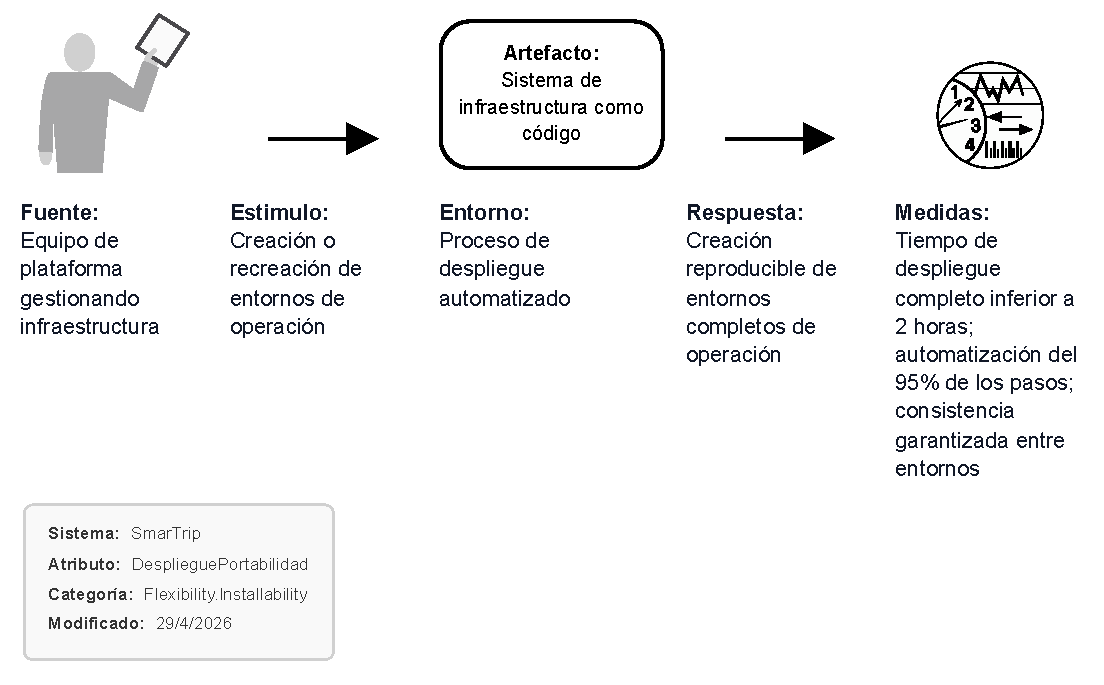
\includegraphics[width=0.85\textwidth,height=0.6\textheight,keepaspectratio]{figures/quality-attributes.SmarTrip_DesplieguePortabilidad.pdf}
    \caption{Despliegue y portabilidad}
    \label{fig:deployment_portability}
\end{figure}

\begin{figure}[H]
    \centering
    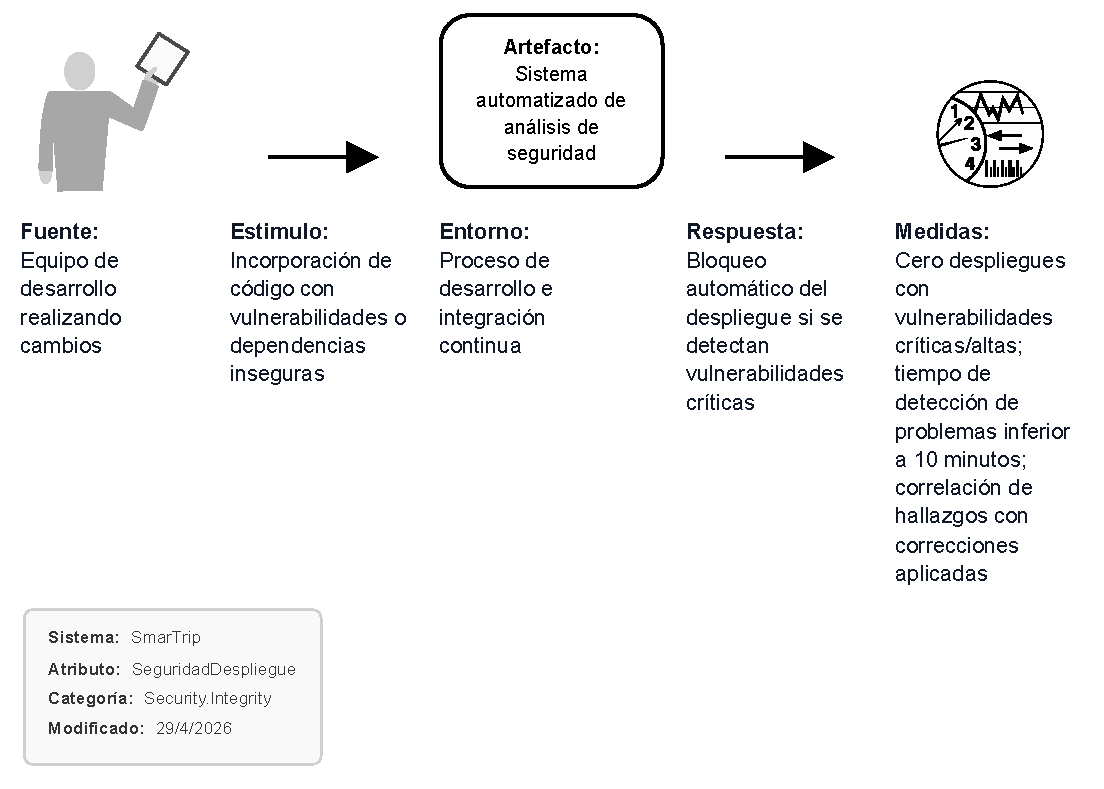
\includegraphics[width=0.85\textwidth,height=0.6\textheight,keepaspectratio]{figures/quality-attributes.SmarTrip_SeguridadDespliegue.pdf}
    \caption{Seguridad en el despliegue}
    \label{fig:deployment_security}
\end{figure}

\begin{figure}[H]
    \centering
    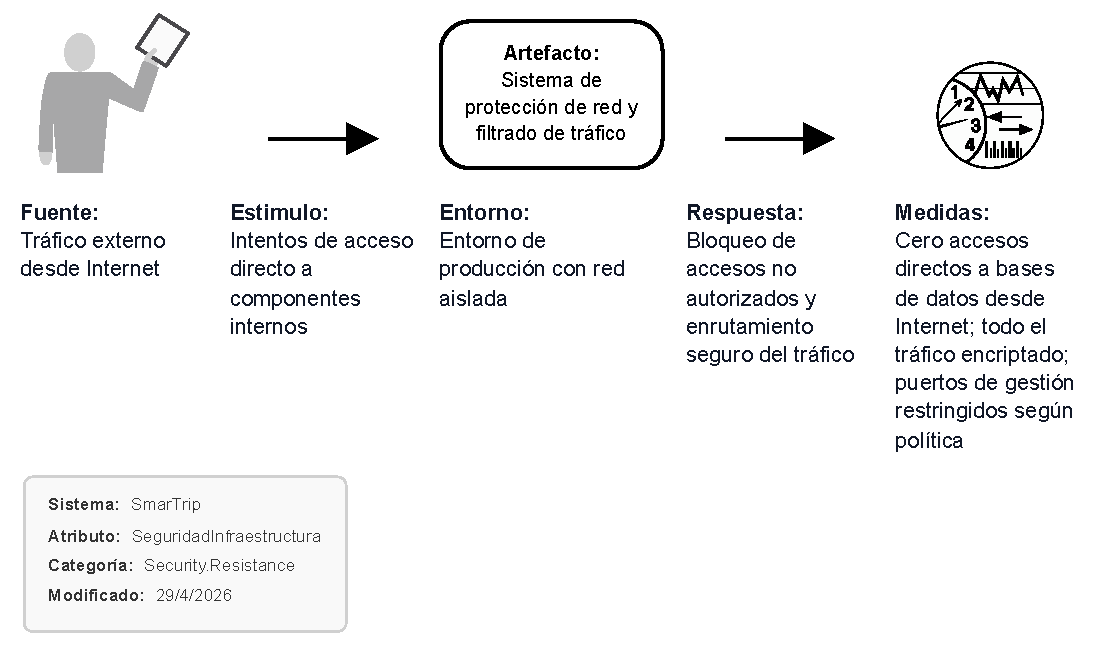
\includegraphics[width=0.85\textwidth,height=0.6\textheight,keepaspectratio]{figures/quality-attributes.SmarTrip_SeguridadInfraestructura.pdf}
    \caption{Seguridad de la infraestructura}
    \label{fig:infra_security}
\end{figure}

%================================================================================
\section{Conclusiones}
%================================================================================

La solución empresarial de transformación digital presentada articula planificación de viajes personalizados y colaborativos con una arquitectura modular verificable en el repositorio de infraestructura. La incorporación de inteligencia artificial, formalizada mediante el modelo PEAS y recomendadores híbridos, justifica técnicamente la separación entre núcleo transaccional (Spring Boot) y microservicio de IA (FastAPI) y su despliegue conjunto detrás de API Gateway y Application Load Balancer.

El estudio argumenta que una arquitectura cognitiva con memorias episódica, semántica y procedimental, combinada con modelos híbridos de recomendación, favorece la personalización y la eficiencia operativa en el turismo regional. El diferencial de \textbf{viaje social colaborativo}---coincidencias, conexiones, mensajería, itinerarios compartidos y evolución hacia \textit{matching} asistido por IA---alinea la solución con la documentación de innovación software del repositorio. La arquitectura cloud-native de referencia en AWS Academy (CloudFront y S3 para el cliente web React, clientes hacia API Gateway, EC2 con autoescalado, RDS PostgreSQL 15.4, S3 para objetos, SNS/SQS y CloudWatch) demuestra viabilidad técnica bajo restricciones de laboratorio y constituye base para endurecimiento y despliegues productivos.

En conjunto, el trabajo evidencia coherencia entre modelo de negocio, requisitos ágiles documentados, componentes de código (web, móvil, backend, IA) e infraestructura como código. La validación empírica futura cuantificará el impacto en Precision@K, tiempo de planificación y mitigación de estacionalidad.

\newpage

\renewcommand{\refname}{Referencias}
\begin{thebibliography}{00}

\bibitem[Colombia Consolida Su Auge Turístico Y Proyecta Cerrar 2025 Con Más De 21,7 Millones De Viajeros, Crecimiento Superior Al 6 \%, n.d.]{ref1}
Colombia consolida su auge turístico y proyecta cerrar 2025 con más de 21,7 millones de viajeros, crecimiento superior al 6 \%. (n.d.). Presidencia De La República. https://www.presidencia.gov.co/prensa/Paginas/Colombia-consolida-su-auge-turistico-y-proyecta-cerrar-2025-con-mas-de-21-7-251201.aspx

\bibitem[Crecimiento Del Turismo Refleja La Consolidación De La Conectividad Aérea Y La Confianza De Los Viajeros | MINCIT, n.d.]{ref2}
Crecimiento del turismo refleja la consolidación de la conectividad aérea y la confianza de los viajeros | MINCIT. (n.d.). MINCIT. https://www.mincit.gov.co/prensa/noticias/turismo/crecimiento-turismo-refleja-confianza-de-viajeros

\bibitem[Informes De Turismo | MINCIT - Ministerio De Comercio, Industria Y Turismo, n.d.]{ref3}
Informes de turismo | MINCIT - Ministerio de Comercio, Industria y Turismo. (n.d.). https://www.mincit.gov.co/estudios-economicos/estadisticas-e-informes/informes-de-turismo

\bibitem[Visitantes No Residentes | Portal De Información Turística De Colombia, n.d.]{ref4}
Visitantes no residentes | Portal de Información Turística de Colombia. (n.d.). https://portucolombia.mincit.gov.co/tematicas/visitantes-no-residentes

\bibitem[De Estadística, n.d.]{ref5}
De Estadística, D. a. N. (n.d.). DANE - PIB Información técnica. https://www.dane.gov.co/index.php/estadisticas-por-tema/cuentas-nacionales/cuentas-nacionales-trimestrales/pib-informacion-tecnica

\bibitem[Staff, 2025]{ref6}
Staff, F. (2025, September 2). Colombia recibió más de 3 millones de turistas en los primeros seis meses del 2025 y alcanzó récord. Forbes Colombia. https://forbes.co/2025/09/02/actualidad/turismo-en-colombia-crece-59-y-rompe-record-este-2025

\bibitem[Instituto Distrital de Turismo (IDT), 2025]{ref7}
Instituto Distrital de Turismo – IDT. (22 de septiembre de 2025). Bogotá superó 1,2 millones de visitantes internacionales entre enero y agosto de 2025. https://www.idt.gov.co/noticias/bogota-supero-12-millones-de-visitantes-internacionales-entre-enero-y-agosto-de-2025

\bibitem[Duque, 2025]{ref8}
Duque, J. S. (2025, March 25). Los desafíos del turismo en Colombia. Report News - Colombia. https://colombia.reportnews.la/blog/2025/03/16/los-desafios-del-turismo-en-colombia/

\bibitem[Balaguera, 2025]{ref9}
Balaguera, P. a. G. (2025, February 20). Despegar: Colombia bate récord de turistas y apunta a consolidarse como destino global. Portafolio.co. https://www.portafolio.co/negocios/empresas/turismo-en-colombia-2025-crecimiento-oportunidades-y-retos-para-el-sector-624281

\bibitem[Box et al., 2015]{ref10} Box, G. E. P., Jenkins, G. M., \& Reinsel, G. C. (2015). \textit{Time series analysis: Forecasting and control}. Wiley.

\bibitem[Ricci et al., 2015]{ref11} Ricci, F., Rokach, L., \& Shapira, B. (2015). \textit{Recommender systems handbook}. Springer.

\bibitem[TOGAF, 2018]{ref12} TOGAF. (2018). \textit{The Open Group Architecture Framework}. The Open Group.

\bibitem[Zhang et al., 2022]{ref13} Zhang, Y., et al. (2022). Deep learning in tourism recommendation systems. \textit{Expert Systems with Applications}, 190.

\end{thebibliography}

\end{document}
